% Template for PLoS
% Version 3.4 January 2017
%
% % % % % % % % % % % % % % % % % % % % % %
%
% -- IMPORTANT NOTE
%
% This template contains comments intended 
% to minimize problems and delays during our production 
% process. Please follow the template instructions
% whenever possible.
%
% % % % % % % % % % % % % % % % % % % % % % % 
%
% Once your paper is accepted for publication, 
% PLEASE REMOVE ALL TRACKED CHANGES in this file 
% and leave only the final text of your manuscript. 
% PLOS recommends the use of latexdiff to track changes during review, as this will help to maintain a clean tex file.
% Visit https://www.ctan.org/pkg/latexdiff?lang=en for info or contact us at latex@plos.org.
%
%
% There are no restrictions on package use within the LaTeX files except that 
% no packages listed in the template may be deleted.
%
% Please do not include colors or graphics in the text.
%
% The manuscript LaTeX source should be contained within a single file (do not use \input, \externaldocument, or similar commands).
%
% % % % % % % % % % % % % % % % % % % % % % %
%
% -- FIGURES AND TABLES
%
% Please include tables/figure captions directly after the paragraph where they are first cited in the text.
%
% DO NOT INCLUDE GRAPHICS IN YOUR MANUSCRIPT
% - Figures should be uploaded separately from your manuscript file. 
% - Figures generated using LaTeX should be extracted and removed from the PDF before submission. 
% - Figures containing multiple panels/subfigures must be combined into one image file before submission.
% For figure citations, please use "Fig" instead of "Figure".
% See http://journals.plos.org/plosone/s/figures for PLOS figure guidelines.
%
% Tables should be cell-based and may not contain:
% - spacing/line breaks within cells to alter layout or alignment
% - do not nest tabular environments (no tabular environments within tabular environments)
% - no graphics or colored text (cell background color/shading OK)
% See http://journals.plos.org/plosone/s/tables for table guidelines.
%
% For tables that exceed the width of the text column, use the adjustwidth environment as illustrated in the example table in text below.
%
% % % % % % % % % % % % % % % % % % % % % % % %
%
% -- EQUATIONS, MATH SYMBOLS, SUBSCRIPTS, AND SUPERSCRIPTS
%
% IMPORTANT
% Below are a few tips to help format your equations and other special characters according to our specifications. For more tips to help reduce the possibility of formatting errors during conversion, please see our LaTeX guidelines at http://journals.plos.org/plosone/s/latex
%
% For inline equations, please be sure to include all portions of an equation in the math environment.  For example, x$^2$ is incorrect; this should be formatted as $x^2$ (or $\mathrm{x}^2$ if the romanized font is desired).
%
% Do not include text that is not math in the math environment. For example, CO2 should be written as CO\textsubscript{2} instead of CO$_2$.
%
% Please add line breaks to long display equations when possible in order to fit size of the column. 
%
% For inline equations, please do not include punctuation (commas, etc) within the math environment unless this is part of the equation.
%
% When adding superscript or subscripts outside of brackets/braces, please group using {}.  For example, change "[U(D,E,\gamma)]^2" to "{[U(D,E,\gamma)]}^2". 
%
% Do not use \cal for caligraphic font.  Instead, use \mathcal{}
%
% % % % % % % % % % % % % % % % % % % % % % % % 
%
% Please contact latex@plos.org with any questions.
%
% % % % % % % % % % % % % % % % % % % % % % % %

\documentclass[10pt,letterpaper]{article}
\usepackage[top=0.85in,left=2.75in,footskip=0.75in]{geometry}

% amsmath and amssymb packages, useful for mathematical formulas and symbols
\usepackage{amsmath,amssymb}

% Use adjustwidth environment to exceed column width (see example table in text)
\usepackage{changepage}

% Use Unicode characters when possible
\usepackage[utf8x]{inputenc}

% textcomp package and marvosym package for additional characters
\usepackage{textcomp,marvosym}

% cite package, to clean up citations in the main text. Do not remove.
\usepackage{cite}

% Use nameref to cite supporting information files (see Supporting Information section for more info)
\usepackage{nameref,hyperref}

% line numbers
\usepackage[right]{lineno}

% ligatures disabled
\usepackage{microtype}
\DisableLigatures[f]{encoding = *, family = * }

% color can be used to apply background shading to table cells only
\usepackage[table]{xcolor}

% array package and thick rules for tables
\usepackage{array}

% create "+" rule type for thick vertical lines
\newcolumntype{+}{!{\vrule width 2pt}}

% create \thickcline for thick horizontal lines of variable length
\newlength\savedwidth
\newcommand\thickcline[1]{%
  \noalign{\global\savedwidth\arrayrulewidth\global\arrayrulewidth 2pt}%
  \cline{#1}%
  \noalign{\vskip\arrayrulewidth}%
  \noalign{\global\arrayrulewidth\savedwidth}%
}

% \thickhline command for thick horizontal lines that span the table
\newcommand\thickhline{\noalign{\global\savedwidth\arrayrulewidth\global\arrayrulewidth 2pt}%
\hline
\noalign{\global\arrayrulewidth\savedwidth}}


% Remove comment for double spacing
%\usepackage{setspace} 
%\doublespacing

% Text layout
\raggedright
\setlength{\parindent}{0.5cm}
\textwidth 5.25in 
\textheight 8.75in

% Bold the 'Figure #' in the caption and separate it from the title/caption with a period
% Captions will be left justified
\usepackage[aboveskip=1pt,labelfont=bf,labelsep=period,justification=raggedright,singlelinecheck=off]{caption}
\renewcommand{\figurename}{Fig}

% Use the PLoS provided BiBTeX style
\bibliographystyle{plos2015}

% Remove brackets from numbering in List of References
\makeatletter
\renewcommand{\@biblabel}[1]{\quad#1.}
\makeatother

% Leave date blank
\date{}

% Header and Footer with logo
\usepackage{lastpage,fancyhdr,graphicx}
\usepackage{epstopdf}
\pagestyle{myheadings}
\pagestyle{fancy}
\fancyhf{}
\setlength{\headheight}{27.023pt}

%\lhead{
\includegraphics[width=2.0in]{PLOS-submission.eps}}
\rfoot{\thepage/\pageref{LastPage}}
\renewcommand{\footrule}{\hrule height 2pt \vspace{2mm}}
\fancyheadoffset[L]{2.25in}
\fancyfootoffset[L]{2.25in}
%\lfoot{\sf PLOS}

%% Include all macros below

\newcommand{\lorem}{{\bf LOREM}}
\newcommand{\ipsum}{{\bf IPSUM}}

%% END MACROS SECTION

%% Additional packages and local edits
\usepackage{footmisc}
\usepackage{multirow}
\usepackage[T1]{fontenc}
%% required the installation of cm-super 55MB - TeX font package (full version) with CM (EC) in Type1 in T1, T2*, TS1, X2 enc

\let\oldmarginpar\marginpar
\renewcommand\marginpar[1]{\-\oldmarginpar[\raggedleft\footnotesize #1]%hv
{\raggedright\footnotesize #1}}
\reversemarginpar

%\setlength{\marginparwidth}{5cm}
\usepackage{caption}
\usepackage{subcaption}
\usepackage{placeins}
\usepackage{xspace} % see http:
%\usepackage{showframe}

\newcommand{\cursedforest}{\textsc{CursedForest}\xspace}
\newcommand{\ranger}{\textsc{Ranger}\xspace}
\newcommand{\randomforest}{\textsc{randomForest}\xspace}
\newcommand{\mtry}{\texttt{mtry}\xspace}
\newcommand{\ntree}{\texttt{ntree}\xspace}

\begin{document}
\vspace*{0.2in}

% Title must be 250 characters or less.
\begin{flushleft}
{\Large
\textbf\newline{\cursedforest - A Random Forest Implementation for ``Big'' and ``Wide'' Data} % Please use "title case" (capitalize all terms in the title except conjunctions, prepositions, and articles).
}
\newline
% Insert author names, affiliations and corresponding author email (do not include titles, positions, or degrees).
\\
Aidan O'Brien\textsuperscript{1,2},
Piotr Szul\textsuperscript{3},
Robert Dunne\textsuperscript{4}, 
Paul Leo \textsuperscript{5},
Emma L. Duncan \textsuperscript{5,6,7},
Natalie A. Twine\textsuperscript{1,8}
Stephanie Li\textsuperscript{9},
James Doecke\textsuperscript{9},
Nick Ellis\textsuperscript{10}, and
Denis C. Bauer\textsuperscript{1,*}
%, with the Lorem Ipsum Consortium\textsuperscript{\textpilcrow}
\\
\bigskip
\textbf{1} Health \& Biosecurity, CSIRO, Sydney, NSW, Australia
\\
\textbf{2} ANU, Canberra, Australia
\\
\textbf{3} Data61, CSIRO, Brisbane, QLD, Australia
\\
\textbf{4} Data61, CSIRO, Sydney, NSW, Australia
\\
\textbf{5} Institute of Health and Biomedical Innovation, Queensland University of Technology, Brisbane, QLD, Australia
\\
\textbf{6} Department of Endocrinology, Royal Brisbane and Women's Hospital, Brisbane, QLD, Australia
\\
\textbf{7} Faculty of Medicine and Biomedical Sciences, University of Queensland, Brisbane, QLD, Australia
\\
\textbf{8} MQ, QLD, Australia
\\
\textbf{9} Health \& Biosecurity, CSIRO, Brisbane, QLD, Australia
\\
\textbf{10} Oceans \& Atmosphere, CSIRO, Brisbane, QLD, Australia
\bigskip

% Insert additional author notes using the symbols described below. Insert symbol callouts after author names as necessary.
% 
% Remove or comment out the author notes below if they aren't used.
%
% Primary Equal Contribution Note
%\Yinyang These authors contributed equally to this work.

% Additional Equal Contribution Note
% Also use this double-dagger symbol for special authorship notes, such as senior authorship.
%\ddag These authors also contributed equally to this work.

% Current address notes
%\textcurrency a Insert current address of first author with an address update
% \textcurrency b Insert current address of second author with an address update
% \textcurrency c Insert current address of third author with an address update

% Deceased author note
%\dag Deceased

% Group/Consortium Author Note
%\textpilcrow Membership list can be found in the Acknowledgments section.

% Use the asterisk to denote corresponding authorship and provide email address in note below.
* Denis.Bauer@CSIRO.au
\end{flushleft}

%\tableofcontents
%\clearpage

% Please keep the abstract below 300 words
\section{Abstract}

Analyses are performed on ever larger datasets with unprecedentedly detailed information per data point. Specifically in genomics, cohort sizes are in the thousands, each comprising of Millions of variants that make up a person's genetic differences. Traditional approaches are unable to cater for this task and even standard implementations using novel compute paradigms, such as Hadoop/Spark, are limited by the finite resource of computer memory on such data. Specifically, Spark ML's supervised machine learning methods suffer from "the curse of dimensionality". That is, they scale well with samples (n) but not with features (p, variants).

We introduce \cursedforest, a tailored implementation of random forests, designed to handle data with extremely large number of variables per sample. We showcase \cursedforest\ to accurately predict ethnicity from whole genome sequencing profiles of 2,500 individuals and 80 million genomic variants each (1000 Genomes Project) in 30 minutes. \cursedforest\ was the only implementation scaling to the full dataset, outperforming other methods on smaller subsets by 80\% or more. We also demonstrate a GWAS-style analysis using  \cursedforest's feature selection approach on an imputed SNP array dataset (2000 x 7 Million) on Bone mineral density (BMD), successfully predicting known BMD-genes as well as identifying novel candidates.  

\cursedforest is included in our earlier variant interpretation package, VariantSpark, allowing it to perform near real-time classification of population-scale patient cohorts in "patients like mine" scenarios, as well as performing GWAS analysis on large unfiltered whole genome sequencing cohorts. 





\linenumbers

\section{Introduction}
The digital revolution is seeing a dramatic increase in data collected about almost every aspect of
life~\cite{Loebbecke2015}.  These datasets are not only growing vertically, by capturing more events, but also
horizontally by capturing more information about these events.  The challenge of big and ``wide'' data is especially
pronounced in the health space where, for example, whole genome sequencing (WGS) technology enables researchers to
interrogate all 3 billion base pairs of the human genome.

Identifying the relevant or disease specific base pair differences between individuals is the focus of genome wide
association studies (GWAS).  These analyses are typically performed on only the most frequently differing base pairs,
termed single nucleotide polymorphisms (SNPs), by applying linear or logistic regression analysis to each SNP
separately~\cite{CCC2007}.  It has since been demonstrated that not taking interactions between SNPs into account
when filtering for potential disease mutations is inadequate~\cite{Manolio2009,Yang2011} and the approach should 
in-fact be extended to interrogating all genomic positions[CITATION WES vs WGS?].

Hence using more sophisticated machine learning (ML) approaches, in particular tree-based models, have been successful
for taking the interaction of variables into account~\cite{Wright.et.al.2016}. In addition, random forests are well
suited for processing ``wide'' genomic data for two reasons.  Firstly, while other machine learning applications have
the propensity to overfit datasets with more features $p$ than samples $n$ (a consequence of the ``curse of
dimensionality''~\cite{Bauer2014, bellman1961adaptive}), decision trees are resistant to overfitting.  Secondly, random
forests are also very easy to parallelise. As the forest is a sum of decision trees, it is possible to grow separate
trees on different processors and combine the trees. 
%See the discussion of the properties of random forests in Section \ref{section:methods}.

The most popular random forest software packages to date are R-based, although it has been reported that current implementations 
do not scale well with increasing feature size~\cite{Wright.and.Ziegle.2016}.  This is despite R now supporting long vectors (length greater
than $2^{31}-1$), and the \randomforest implementation in R lending itself to parallelisation by growing multiple
trees simultaneously and combining them for the final result~\cite{Liaw.and.Weiner.2002}.  More suitable implementations for ``wide''
genomic data have been developed in other programming languages. \textsc{CloudForest} \cite{Bressler2015}, written in Go,
achieves fast run times by effective use of the CPU cache, optimising for different classes of features and efficiently
multithreading.  Similarly, \ranger~\cite{Wright.and.Ziegle.2016}, written in C++ with an R front-end, is
specifically optimised for dealing with large datasets.

However, the use of traditional compute infrastructure limits the parallelisation strategies that can be employed.  
The programs are limited to utilising only CPUs that are on the same computer node (multithreading) or
farm out independent tasks to CPUs distributed across nodes that do not require communication between the
processes (a separate tree is grown on each node).
%else they can run on CPUs distributed across nodes by virtue of the fact that there is no communication between the
%processes (a separate tree is grown on each node).  
Hadoop/Spark overcomes these limitations by enabling programs to
scale beyond compute-node boundaries and hence enable more sophisticated parallelisation strategies.  In the case of
random forests, the computations for each node of a tree can hence be handed off to separate processors.
 
Despite overcoming the node-boundary limitation, the standard implementation of random forest in Spark ML
is not able to handle the extremely ``wide'' genomic data as it was developed for a large number of samples
with only modest dimensionality~\cite{NIPS2016_6366}.  Although Spark ML can build a random forest model on a subset of the data (chromosome
1), we show that the time taken is excessive due to the large amount of data being aggregated and processed by the driver node during
intermediate stages of building the model.  This unbalanced work load where the driver
node becomes the bottleneck and worker nodes being idle prevents a seamless scaling to larger datasets. We also show that the memory
requirements per executor increases with dimensionality due to the data types Spark ML uses.%, which we elaborate on in the discussion.
  
Here we introduce \cursedforest, a tailored Hadoop/Spark-based implementation of random forests specifically designed to cater
for ``big'' (many samples) and ``wide'' (many features) datasets. 
\cursedforest extends our previously developed variant interpretation framework, VariantSpark~\cite{OBrien2015}, to now offer
supervised as well as unsupervised ML algorithms in the Spark framework.
In our implementation a Spark application runs on a ``driver'' node and
distributes tasks to many ``worker'' nodes, or ``executors''. 
By also utilising Spark to read in and manipulate the standard genomic variant format (VCF)
directly, \cursedforest outperforms existing tools even on small datasets where multithreading generally performs
well. Harnessing the virtually unlimited capability to parallelise tasks, \cursedforest can hence explore the solution 
space faster by building a larger number of diverse models to generate a consensus from. 

Using this facility, \cursedforest is capable of parallelising the split for each node in a tree thereby handling millions 
of features, as required to process whole genome sequencing data or SNP array data with unobserved genotypes 
imputed~\cite{Howie2012}.  This provides the potential to generate datasets of hundreds of thousands of individuals 
with millions of variants (imputing the GWAS catalog), highlighting the need for modern
compute paradigms in the genomics space.

%It can, for example, fit a model to the 1000 Genomes Project data, which consists of approximately 2500 samples with up to 80 million
%variants~\cite{1KG2012}.  
%build a larger number of
%trees hence building a larger number of diverse models to generate the consensus from.  %and use a high \mtry value which may lead to greater accuracy (see the example in section \ref{section:synthetic}). 
%\marginpar{does \cite{Szymczak2016} say that high \ntree gives greater  accuracy for variable importance selection?
%Check this. }
%We previously demonstrated the versatility and scalability of Spark by developing VariantSpark~\cite{OBrien2015}, a
%framework allowing users to easily analyze Variant Call Format (VCF) files using ML algorithms on the Spark framework.
%Using VariantSpark, we successfully built a k-means model on the full $2500 \times 80$ million matrix to cluster
%individuals by their ethnicity achieving an Adjusted Rand Index (ARI) of 0.84 (with 1 being perfect clustering and -1
%random clustering).
%Using VariantSpark, we successfully built a k-means model on the full $2500 \times 80$ million matrix to cluster
%individuals by their ethnicity achieving an Adjusted Rand Index (ARI) of 0.84 (with 1 being perfect clustering and -1
%random clustering).
%Here we extend this toolkit to encompass supervised learning using random forests.  

VariantSpark~\cite{OBrien2015} with the \cursedforest extension therefore offers a
comprehensive analysis toolkit that can scale to future data demands. To showcase the framework's ability we demonstrate
a classification as well as feature-selection task on synthetic data in the first section. In the second section, we demonstrate the ability of
\cursedforest to successfully replicate findings from a previous GWAS study as well as identify novel variants associated with bone 
mineral density (BMD). 
Thirdly, we demonstrate the scalability of \cursedforest in respect to the dimensionality of data by building a random
forest model on whole-genome data from the 1000 Genomes Project~\cite{1KG2012} to predict ethnicity.
Finally, given the role different parameter values can play in model construction, we explore the effect that tuning these
parameters can have on the prediction accuracy of the model.



\section{Methods}
\label{section:methods}

%%%%%%%%%%%%%%%%%%%%%%%%%%%%%%%%%%%%%%%%%%%%
\subsection{Overview of Random Forests}

Decision trees have a number of desirable features, they:
\begin{itemize}
  \item are invariant to monotonic scaling of the data;
  \item can handle categorical and real valued inputs;
  \item can handle missing values;
  \item are insensitive to uninformative predictors;
  \item are able to capture interactions between features (which is important for modeling complex polygenic diseases).
  \end{itemize}
However, the tree fitting algorithm is greedy and may generate an unstable model. That is, a small change in the data may
lead to a very different model. 

Random forests apply the technique of bootstrap aggregation or bagging to decision trees.  The training datasets are
independently drawn, with replacement, from the joint distribution of $(X,Y)$ so that each set comprises $n$
$(p+1)$-tuples $(x_1,y_1),\ldots, (x_n,y_n)$. This is done $B$ times and a tree is grown on each of these $B$ samples.
The results are then combined in an appropriate way. In a classification problem we take the majority vote for the trees
over the $q=1,..,Q$ classes,
\begin{equation*}
{{h_f}}= \arg \max_q \left(\sum_b I(h(x;B_b)=q)\right).
\end{equation*}
In addition to growing the trees
on bootstrapped samples, each node in the tree is split on a randomly
selected subset of the variables.

Random forests are a variance reduction technique. They take unpruned tree models, which have a low bias but a high
variance, and by combining them reduce the variance.  For regression problems, as the prediction error is the sum of the
variance and the bias squared, this strategy should lead to a low prediction error.

For classifiction problems there is no obvious decomposition of classification error into an equivalent bias plus
variance form. A number of different additive decompositions of classification error have been considered in an effort
to understand the success of bagging. They are all less transparent than the regression case (see \cite{Friedman.1997} and
citations therein).

In the case of a regression tree, the average prediction error for an individual tree $h(X; B)$ is
\begin{equation}
PE_t = E_B E_{X,Y} (Y-h(X; B))^2.
\end{equation}
Assume that, for all $B$, the tree is unbiased, i.e., $EY= E_X h(X; B)$. Then
\begin{equation}
PE_f \leq \rho PE_t
\end{equation}
where $\rho$ is the weighted correlation between residuals $(Y-h(X;B))$ and $(Y-h(X;B^\prime))$ for independent
$B,B^\prime$.
So what is required for accurate random forest regression is (i) low correlation between residuals of differing tree in
the forest, and (ii) low prediction error for the individual trees \cite{Segal.2004}. 

The benefits of random forest models are:
\begin{itemize}
\item they give an out-of-bag (OOB) estimate of model accuracy, by using the samples not selected for the bootstrapped sample
  as an independent test set for each tree;
\item they provide a measure of variable importance, for example by summing the number of times a variable is used to
  split a node, over all nodes and all trees. More complex measures of variable importance are also used;
\item they inherit some of the qualities of tree models (but not, for example, the handling of missing values via surrogate
  variables. This would be difficult as the trees are split on random subsets of variables).
\end{itemize}

Since the original implementation of random forests, there have been a number of developments leading to a better
understanding of the algorithm.
\begin{itemize}
\item random forests are resistant to overfitting. However it is not true that they will not overfit,
  ~\cite{Segal.2004} gives examples of overfitting in cases where:
  \begin{itemize}
  \item a single tree is the most appropriate model; and
  \item the variables are highly correlated so that the bootstrap resampling does not give rise to uncorrelated trees.
  \end{itemize}
However, keeping these difficult cases in mind, random forests have a strong claim to being resistant to overfitting.
\item \cite{Strobl.et.al.2007} demonstrates that the random forest algorithm is subject to a bias in variable selection
  via two mechanisms:
  \begin{enumerate}
  \item differences in variable scale (for $X_i$ continuous) and number of levels (for $X_i$ discrete) introduces a
    bias. An uninformative variable with a large number of levels may be selected over a more informative variable with
    fewer levels;
  \item bagging introduces a bias, but sampling $(1- 1/e) \approx 0.632$ of the data without replacement seems to be an
    effective strategy for removing the problem.
  \end{enumerate}
\end{itemize} 

\cite{Strobl.et.al.2007} introduce changes to the random forest algorithm to fix 1) and 2).  Effect 1) will be apparent
in the \cursedforest algorithm as well.  However, there are many examples, particularly in genomics, where we have data
sets that are:
\begin{itemize}
\item very wide;
\item all variables have the same number of levels (for example, measurements at different points along the genome);
\item the hypothesized functional relationship is of a form amenable to a decision tree.
\end{itemize}
GWAS datasets are an obvious application area for this algorithm. 

\cite{Biau.2012} provides a proof that a random forest model will converge at a rate that depends on
the cardinality of the set $S$ of ``strong predictors'' rather than on the number of variables $p$. That is, given a
function $y=f(S)$ depending on a set of variables $S$, a random forest will converge to the true function $y$ with a
rate that depends on the size of $S$ and not the number of noise variables in the dataset. If the size of $S$ is small
compared to the total number of variables, then the rate of convergence will be quicker. It is not clear what the size
of the set $S$ will be in a GWAS application. There are cases of small groups of SNPs with large effects and also of
conditions caused by the interactions of large groups of SNPs.

\cite{Genuer.et.al.2010} and \cite{Diaz.and.Alvarez.2006} describe iterative schemes for doing variable selection using
the importance measure. See \cite{Chen.and.Ishwaran.2012} for a review of the area with particular reference to genomic
data.

%%%%%%%%%%%%%%%%%%%%%%%%%%%%%%%%%%%%%%%%%%%%%%%%%%%%%%%%%%%
\subsection{\cursedforest}
VariantSpark made use of Spark's machine learning algorithms ``Spark ML''. While Spark ML algorithms demonstrate
scalability when dealing with a large number of samples, this scalability eventually breaks down as we include more
features.

As is standard with Spark applications, we store our data in a Resilient Distributed Dataset (RDD), where an RDD is
essentially a collection of elements. In the case of Spark ML, each element in the RDD is a sample. RDDs contribute to
the scalability of Spark as they can be distributed across multiple nodes and operated on in parallel. Even as we add more
samples to a dataset, Spark can simply schedule extra tasks to handle the additional items in the RDD.

However, within an RDD, Spark ML stores each sample as a vector. Unlike RDDs, which can be partitioned and distributed
across multiple nodes, each vector must be present in its entirety on any node accessing it. This is no problem with
typical datasets; however as dimensionality increases, the vectors eventually reach a size where they can no longer fit
into a single node's memory.

So in the case of adding more samples, Spark ML can simply create more tasks, keeping memory consumption within the
cluster's bounds. However, as the dimensionality of each sample grows, the memory requirements of the job increases to
enable these increasingly large vectors to be loaded into memory.  

On the other hand, \cursedforest is specifically designed to handle wide ``cursed'' data. It avoids the relation between
memory and dimensionality by avoiding calculations that rely on entire feature vectors and taking the parallelization
work down to the level of the individual features.  For each node of a tree, \cursedforest will distribute
tasks that consist of single features (variants), for every individual.  Each of these tasks will calculate the
information gain for that specific feature.  Once these tasks have completed, the results are reduced to return the
feature which gives the greatest information gain.  This process is then repeated until \cursedforest has created the
entire decision tree.

The current implementation of \cursedforest uses a ``Gini impurity'' criteria for splitting. Let $f_q$ be the fraction
of items labeled with value $q$, where $q = 1, \ldots, Q$ at a node. The Gini impurity is
$$
I_G(f) = \sum_{q = 1}^Q f_q ( 1 - f_q ), 
$$
which is at a minimum when all observations at the node are in the same class.

%%%%%%%%%%%%%%%%%%%%%%%%%%%%%%%%
% This section talks about the datasets
%%%%%%%%%%%%%%%%%%%%%%%%%%%%%%%%
\subsection{Datasets}
\subsubsection{1000 Genomes Project}
We obtained the 1000 Genomes Project data as VCF files from their FTP site.  Each VCF file contains the variants for
every individual across one chromosome.  We use the phase 3 dataset which contains 2,504 individuals with approximately
81 million variant positions (i.e. a matrix of $2,504 \times 81$ million).  For compatibility with the majority of the
algorithms we demonstrate, we convert the original variant representations to double representations.  For example, we
store the absence of a variant (0\textbar0) as 0, a heterozygous
variant (1\textbar0 or 0\textbar1) as 1, and a
homozygous variant (1\textbar1) as 2.  However, this is not the only possible encoding \cite{Goldstein.et.al.2011}. Note that from
the encodings listed in Table~\ref{table:encodings}, the additive encoding will present the most difficulty for a random
forest model.


\begin{table}[!ht]
%\begin{adjustwidth}{-2.25in}{0in} % Comment out/remove adjustwidth environment if table fits in text column.
\begin{flushleft} 
\centering
\caption{\bf Possible encodings of GWAS data \cite{Goldstein.et.al.2011}}
\begin{tabular}{|l|l|l|l||}
\hline
{\bf Type} & {\bf Mechanism}                                         & {\bf Partition} \\ 
\thickhline
Additive   & Each additional minor allele increases variation        & 0, 1, 2         \\
Dominant   & Presence of at least 1 minor allele increases variation & 0, $\{1,2\}$          \\
Recessive  & Two minor alleles needed for variation                  & $\{0,1\}$, 2          \\
Heterosis  & Heterozygote leads to variation                         & $\{0,2\}$, 1          \\ \hline
%\end{adjustwidth}
\end{tabular}
\label{table:encodings}
\end{flushleft}
\end{table}


\subsubsection{Bone mineral density dataset}
We obtained a VCF file from the authors of \cite{Duncan.2011}, which contains variant data from 1,936 postmenopausal women.
This dataset covers approximately 7 million variant positions. We have information about the bone mineral density (BMD)
for each individual, where a low BMD is a major predisposing factor to fracture \cite{Duncan.2011}. 

\subsubsection{Synthetic data} 
\label{section:synthetic_data}
 Each dataset consists of $n$ samples and $p$ variables where $n << p$,
and values for each variable are ordinal variables with three levels represented as numbers $\{0, 1, 2\}$ (which
correspond to an additive effect encoding of genomic variation) randomly generated from a uniform distribution with equal
probabilities.  

The model parameters are $w_i = 1/\sqrt{2^{i-1}}$ for $i =1,\ldots 5$ and we set 
\begin{equation}
\label{equation:synthetic.data}
z =  \sum_{i=1}^{i=5} {w_i x_i}.
\end{equation}
We let $\sigma_\epsilon^2 = Var(z)(1-\theta)/\theta $  where $\theta$ is a parameter controlling the fraction of variance explained by the informative variables and in our study we chose $\theta = 0.125$ . Then 
$y =   z + \epsilon$ where $\epsilon \sim  N(0, \sigma_\epsilon^2).$
The dichotomous response is generated by thresholding $y$ at the $0.5$ quantile.

$$
\ddot{y} =    \left\{ \begin{array}{rcl}
			  0 & \mbox{for} & y \leq Q2(y) \\
			  1 & \mbox{for} & y > Q2(y)
		 \end{array}\right.
$$


\subsection{Parameter settings}
We consider the parameter settings for the random forest algorithm. We use the R notation from the \randomforest
package \cite{Liaw.and.Weiner.2002} which incorporates the original Fortran code by Brieman and Cutler.  We incorporate
the advice of \cite{Liaw.and.Weiner.2002}, which we have found mirrors our own experience:
\begin{itemize}
\item \ntree{}  -- the number of trees.  The number of trees necessary for good performance grows with the number of
  predictors.  \cite{Liaw.and.Weiner.2002} suggest that a high \ntree is necessary to get stable estimates of variable
  importance and proximity; however, even though the variable importance measures may vary from run to run, we note that
  it is possible for a random forest model to have a poorer fit and still have an accurate ranking of variable
  importance;
\item \mtry{}  -- the number of variables considered at each split (if \mtry=$p$, we have a boosted decision
  tree model).  If one has a very large number of variables but expects only very few to be ``important'', using larger \mtry may give
  better performance;
\item the size and complexity of the individual trees is controlled in \randomforest by setting \texttt{nodesize}, the
  minimum size of terminal nodes. It is controlled in Spark ML by setting \texttt{maxDepth}, the maximum depth of each
  tree in the forest.\footnote{The Spark ML documentation \cite{Spark.2016} sets \texttt{maxDepth} to 4 in their
    classification example. This may give an estimate with a higher bias and, as such, may be a poor choice. See the
    discussion in \cite{Dietterich.2002} where it is shown that bagging may reduce bias as well as variance but is more
    complicated than first thought. They show that bagging may reduce bias as well as variance but give a    
    better result for low bias learners. \cite{Dietterich.2002} notes that if the bootstrap replicate approximation were
    correct (i.e.~if the bootstrap sample came from an identical distribution to the data), then bagging would reduce
    variance without changing bias.}
\end{itemize}



%%%%%%%%%%%%%%%%%%%%%%%%%%%%%%%%
%
% Results
%
%%%%%%%%%%%%%%%%%%%%%%%%%%%%%%%%
\section{Results and Discussion}


%%%%%%%%%%%%%%%%%%%%%%%%%%%%%%%%
% Section 2: Feature Selection on real data 
%%%%%%%%%%%%%%%%%%%%%%%%%%%%%%%%
%\subsection{GWAS-style analysis using \cursedforest\ identifies novel variants associated with Bone Mineral Density}
\subsection{GWAS-style analyses using \cursedforest\ faithfully identify known disease-accociated genes}
In this section we use \cursedforest\ to perform feature selection on over 7.2 million genomic variants and identify the
genomic locations associated with Bone Mineral Density (BMD)~\cite{Duncan.2011}. 
%We build a model on the BMD dataset as described in Methods using a binary high or low BMD value as the label.  
We rank variants by their Gini impurity, with the most important one ranked at position 1, and return the top 100,000 variants.

To test whether the associated variants have biological meaning, we investigate if variants in or near
BMD-associated genes are enriched toward the top of our ranked list. To form the list of "known genes", we
combine the 26 known and 6 novel BMD genes listed by Duncan {\it et al.}~\cite{Duncan.2011} with the genes identified by
Estrada {\it et al.}~\cite{Estrada2012} and Lui {\it et al.}~\cite{Liu2008}, resulting in 102 genes.  All genes are covered within the
top 40,000 variants and a gene name is assigned to the variant if it falls within 100 kb of this gene.

The known genes rank significantly higher than variants from other locations in the genome (Mann-Whitney U, $p=4.5\times10^{-14}$, Supplemental File 1), 
supporting our hypothesis that biologically relevant features are contributing more information to our classification model.

%~\ref{figure:BMDTopWholeGenome}, 
As shown in Figure 1a, the top 30 features are dominated by variants from five well established BMD genes; TNFRSF11B (TNF Receptor Superfamily Member 11b or Osteoprotegerin), CTNNB (Catenin Beta 1), ZBTB40 (Zinc Finger And BTB Domain-Containing Protein 40), IBSP (Integrin Binding Sialoprotein) and MEF2C (Myocyte Enhancer Factor 2C). 
The BMD association has been independently replicated for four of the five genes: TNFRSF11B~\cite{Rivadeneira2009,Zhang2014,Kemp2014,Paternoster2013}, CTNNB1~\cite{Pei2016, Rivadeneira2009}, ZBTB40~\cite{Rivadeneira2009,  Zhang2014,Nielson2016}, and MEF2C~\cite{Pei2016a}. 
The association of IBSP has not been replicated in other GWAS studies, but homozygous knockouts of this gene have a known skeletal phenotype in mice. Mice deficient in IBSP have impaired bone growth and mineralization, with dramatically reduced bone formation~\cite{Malaval2008}. 
CTNBB1, MEF2C and TNFRSF11B also have known skeletal phenotypes. 
CTNNB1 is a key downstream member of the Wnt signaling pathway, and deletion of CTNNB1 in mice results in severe osteopenia, while constitutive activation of CTNNB1 results in massively increased bone deposition~\cite{Holmen2005}. 
MEF2C is a transcription factor which controls bone mass by regulating osteoclastic bone resorption, where mice with a MEF2C deletion in osteocytes had increased bone mass compared with normal controls~\cite{Kramer2012}. TNFRSF11B (or OPG) is a secreted glycoprotein which regulates bone mass~\cite{Simonet1997}. 
ZBTB40 has no known biological or molecular involvement in skeletal phenotypes~\cite{Styrkarsdottir2008}, even though it has been associated with BMD in multiple GWAS and is expressed in bone.
SNPs in linkage disequilibrium (LD) with each other at these loci also show a high importance score, as exemplified by TNFRSF11B in Figure 3b (Supplemental Figure 2 and 3 for the other genes). %~\ref{manhattenzoom}).

%MAPT microtubule associated protein tau \cite{Dengler-Crish2017}
%"MAPT is primarily expressed in the nervous system and has not been identified in bone tissue, therefore, low BMD in a tauopathy-specific mouse model that lacks A? pathology would provide evidence that central mechanisms of bone homeostasis are dysfunctional in AD, rather than only direct peripheral effects on bone tissue itself."
%"Reduced bone mineral density (BMD) and its clinical sequelae, osteoporosis, occur at a much greater rate in patients with Alzheimer?s disease (AD), often emerging early in the disease before significant cognitive decline is seen. "

In contrast, one of the lowest ranked gene with literature implied BMD association is DCDC5 (Doublecortin Domain Containing 5) ranked 23,842
(see Supplemental Figure 1). Similar to the conclusions drawn by Duncan {\it et
  al.}~\cite{Duncan.2011}, our results also indicate that this gene does not have a strong association with BMD. DCDC5 is not highly expressed in bone, and any mechanisms by which this gene might regulate BMD are unclear
\cite{Thakker2012}.  Although variants near DCDC5 are associated with BMD \cite{Rivadeneira2009}, it is questionable as
to whether the gene itself contributes to BMD.
Similarly, the lowest ranked gene with annotated BMD links, MAPT (microtubule associated protein tau) at 36,262, is primarily expressed in the nervous system and has not been identified in bone tissue. 
It is therefore likely that the association is through a co-morbidity with Alzheimer's disease~\cite{Dengler-Crish2017} and not a major contributing factor in this cohort. 


\subsection{\cursedforest\ amplifies signal over traditional methods to identify novel associations}

Figure 1b shows a traditional GWAS analysis using logistic regression~\cite{Duncan.2011} where the resulting $p$-values do not clearly distinguish these known BMD genes from the noise. 
In contrast, \cursedforest\ seems to amplify the signal to identify associated features (Figure 1a). 
As such, this approach allows to employ a very stringent cut-off for identifying strongly associated feature. Here we chose a 99.98 False Discovery Rate (FDR) from 60 random experiments (see Methods). 

%2 TEX2  EN rs112558362 SNORNA  ERN1 Gliablastoma in older people Alzheimer's
%5 rs6961378  Woolfe2005
%13 rs17195090

Above this FDR cut-off we identify four novel locations as annotated in Figure 1a.
%~\ref{figure:rbo-prod.png}. 
Most notably a lincRNA (LINC01006) on chromosome 7, which has been associated with serum creatinine levels in two independent GWAS studies~\cite{Pattaro2010,Chambers2010}. 
Subjects with low serum creatinine levels were at a higher risk for low BMD~\cite{Huh2015} and in a rat study high creatine monohydrate diet resulted in greater lumbar BMD~\cite{Antolic2007}, 
with creatinine being the breakdown product of creatine. The variants overlapping the 5' end of the lincRNA are the highest ranked features in this region and all LD SNPs also show high importance (see Fig 3d). Also amonst the top 30 features is PRODH (proline dehydrogenase) located on 22q11, a loci observed by Stagi {\it
  et al.}~\cite{Stagi.2010} to significantly reduce bone mass in individuals with a micro-deletion in this region. 
PRODH catalyses the first step in proline degradation, and as proposed by Phang {\it et al.}~\cite{Phang.2008}, proline is made available by collagen degradation. 
Again, all LD SNPs also show high importance (see Figure 3c). %~\ref{zoomplot}). 
%Ranked at position 5 (rs6961378) and 18 (rs146034056) are located on chromosome 7 overlapping the lincRNA (LINC01006), which as been linked to vertebrate development~\cite{Woolfe2005}.
In contrast rs17195090 and rs112558362 are single feature loci (Supplementary Figure 4) hence likely due to erroneous imputation or genotyping.

To evaluate whether the here identified features are significantly associated with BMD, we train a traditional linear mixed model to return a $p$-value for each included feature. Interestingly, while the three known BMD genes with the highest Importance score are indeed significantly associated (TNFRSF11B $p$-value=XX, CTNNB1 XX, ZBTB40 XX), IBSP and MEF2C were not significant. All of our newly associated features, on the other hand, were deemed significant, and in-fact rs17195090 was the most significant feature evaluated with $p$-value=XX (rs112558362 XX, LINC01006 XX, PRODH XX). 

% Also amongst the top 20 associated
%variants is a SNP in the intronic region of Unc13c (rs12916554), a gene that is linked to quality of
%sleep~\cite{Nicod2016}, which in turn is reported to be the best predictor of osteoporosis risk~\cite{Magali2016}, a
%condition diagnosed by measuring BMD.  Also listed is rs1035665, which was identified in a recent GWAS study to regulate
%ABCF1 (ATP Binding Cassette Subfamily F Member 1)~\cite{Dixon2007} with member 2 of this subfamily being a known BMD
%gene. The other three novel loci are on or near ncRNA.

%\cursedforest\ can successfully perform GWAS-type analyses replicating previous findings and uncovering novel associations due to random forests also modelling interacting features.

%In Table~\ref{featuretable}, we display the top 10 features, ranked by their Gini impurity measure in the random forest model.

%\begin{table}[!ht]
%%\begin{adjustwidth}{-2.25in}{0in} % Comment out/remove adjustwidth environment if table fits in text column.
%\centering
%\caption{
%{\bf Features from the TCGA BRCA dataset ranked by their importance.}}
%\begin{tabular}{|l|l|l|l|l|l|l|}
%\hline
%{\bf Variant} & {\bf Gene} & {\bf Importance}\\ \thickhline
%8:120003727 & COLEC10 & 1.6393260970E-6\\ \hline
%1:22702231  & ZBTB40  & 1.3901355155E-6\\ \hline
%22:18923745 & PRODH   & 1.3769982791E-6\\ \hline
%1:22702187  & ZBTB40  & 1.3350582926E-6\\ \hline
%3:41111035  & CTNNB1  & 1.2707227479E-6\\ \hline
%1:693731    &         & 1.1786957578E-6\\ \hline  
%1:22700351  & ZBTB40  & 1.1547011076E-6\\ \hline
%8:120040181 & COLEC10 & 1.1511986773E-6\\ \hline
%1:22701761  & ZBTB40  & 1.1495539020E-6\\ \hline
%3:41120417  & CTNNB1  & 1.1325242379E-6\\ \hline
%\end{tabular}
%\begin{flushleft} 
%The ten genes proximal to the top variants as ranked by their Gini impurity from a random forest model built on
%individuals using high/low bone mineral density as the label.
%\end{flushleft}
%\label{featuretable}
%%\end{adjustwidth}
%\end{table}

%\begin{figure}[tbhp]
%  \begin{adjustwidth}{-2.00in}{0in}
%    \caption{\textbf{Rank of literature assigned BMD genes}}
%    \label{figure:knowngeneranks}
%    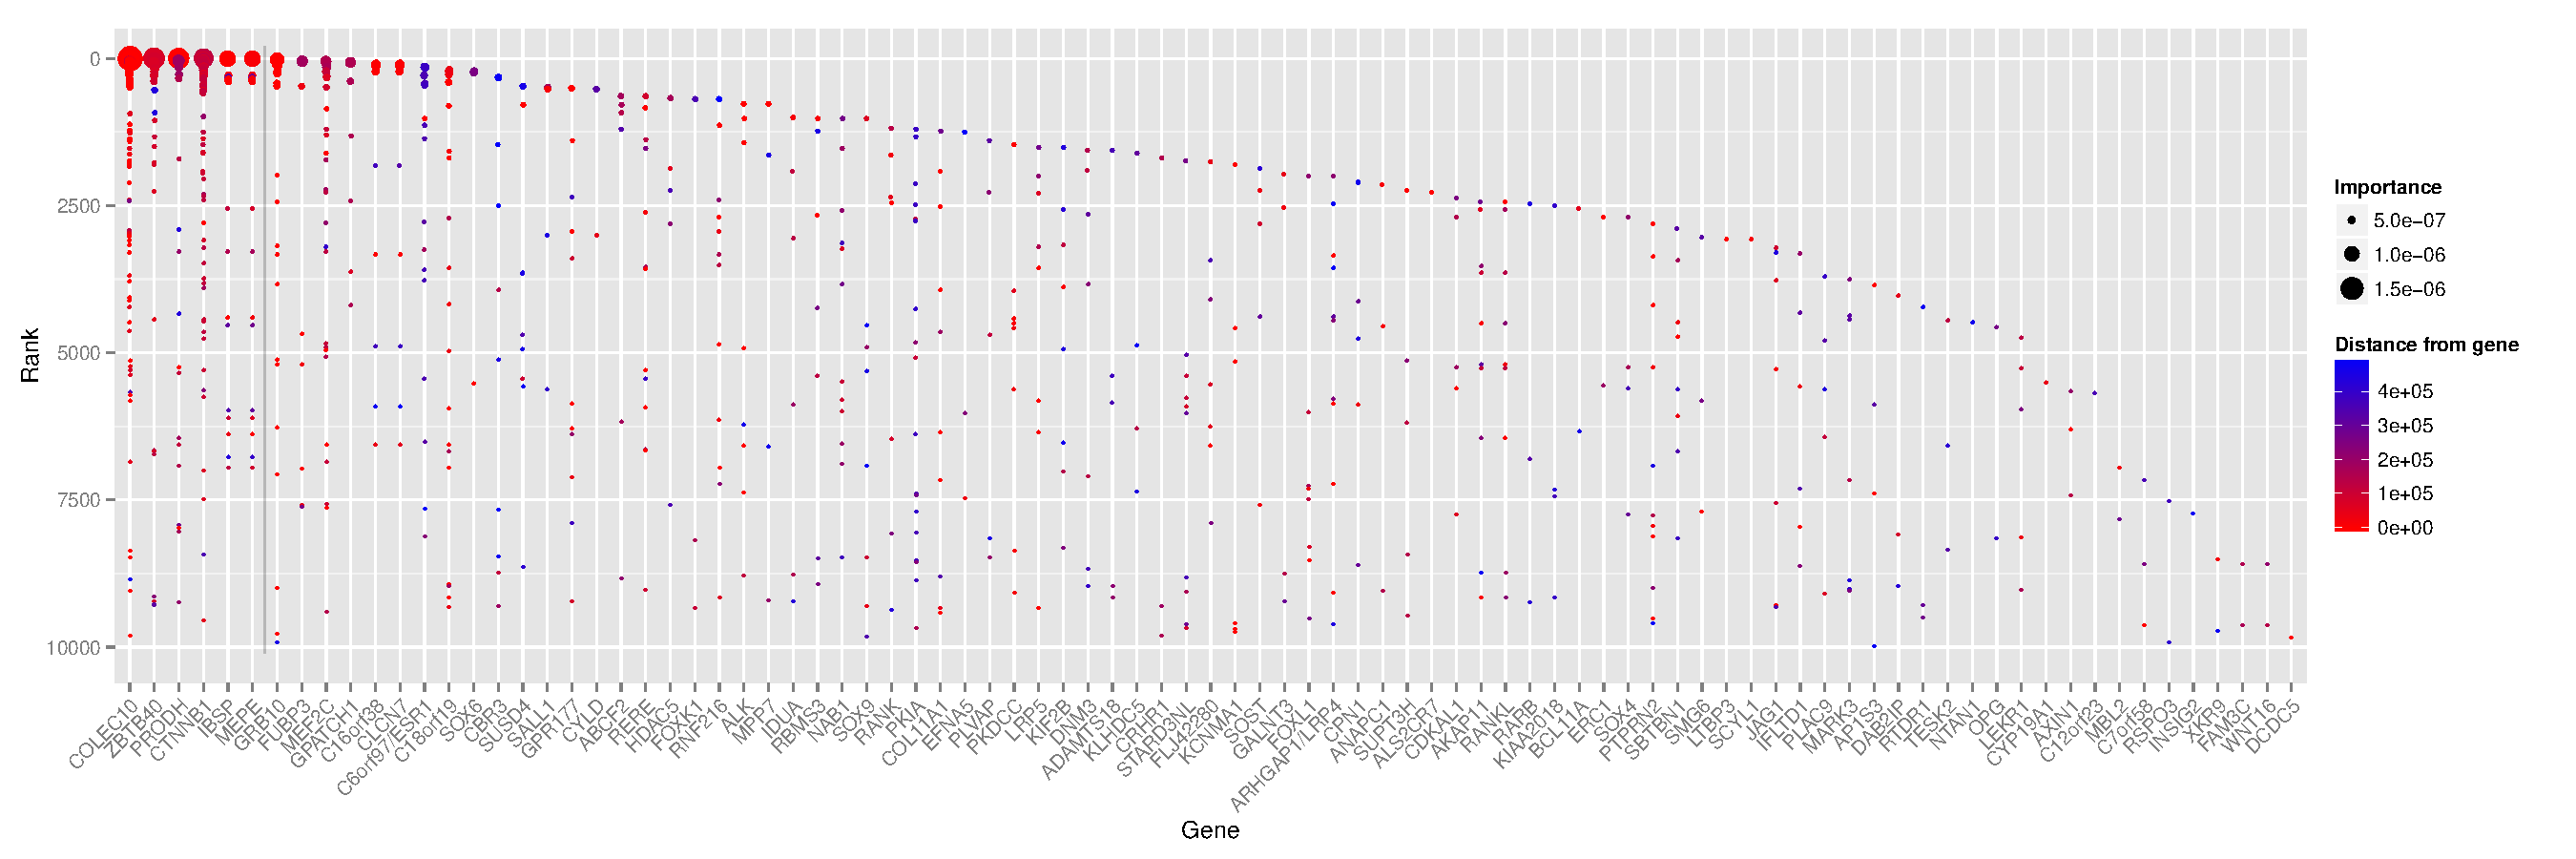
\includegraphics[totalheight=6.5cm]{./figs/BMDgenes_landscape.pdf}
%    \begin{flushleft}
%      The figure shows the rank of the 100 literature assigned BMD genes. Each ball represents a SNP assigned to the closest gene with colour representing the distance (max 100 kb). The size shows the Gini impurity score with larger balls representing more important SNPs. The horizontal line separates the genes with SNPs amongst the Top 20 associated features. 
%     \end{flushleft}
%  \end{adjustwidth}
%\end{figure}


\begin{figure}[tbhp]
  \begin{adjustwidth}{-2.00in}{0in}
    \caption{\textbf{Genome-wide importance of SNPs for Bone Mineral Density association}}
    \label{figure:ranksumtest}
     \begin{subfigure}[b]{0.5\linewidth}
     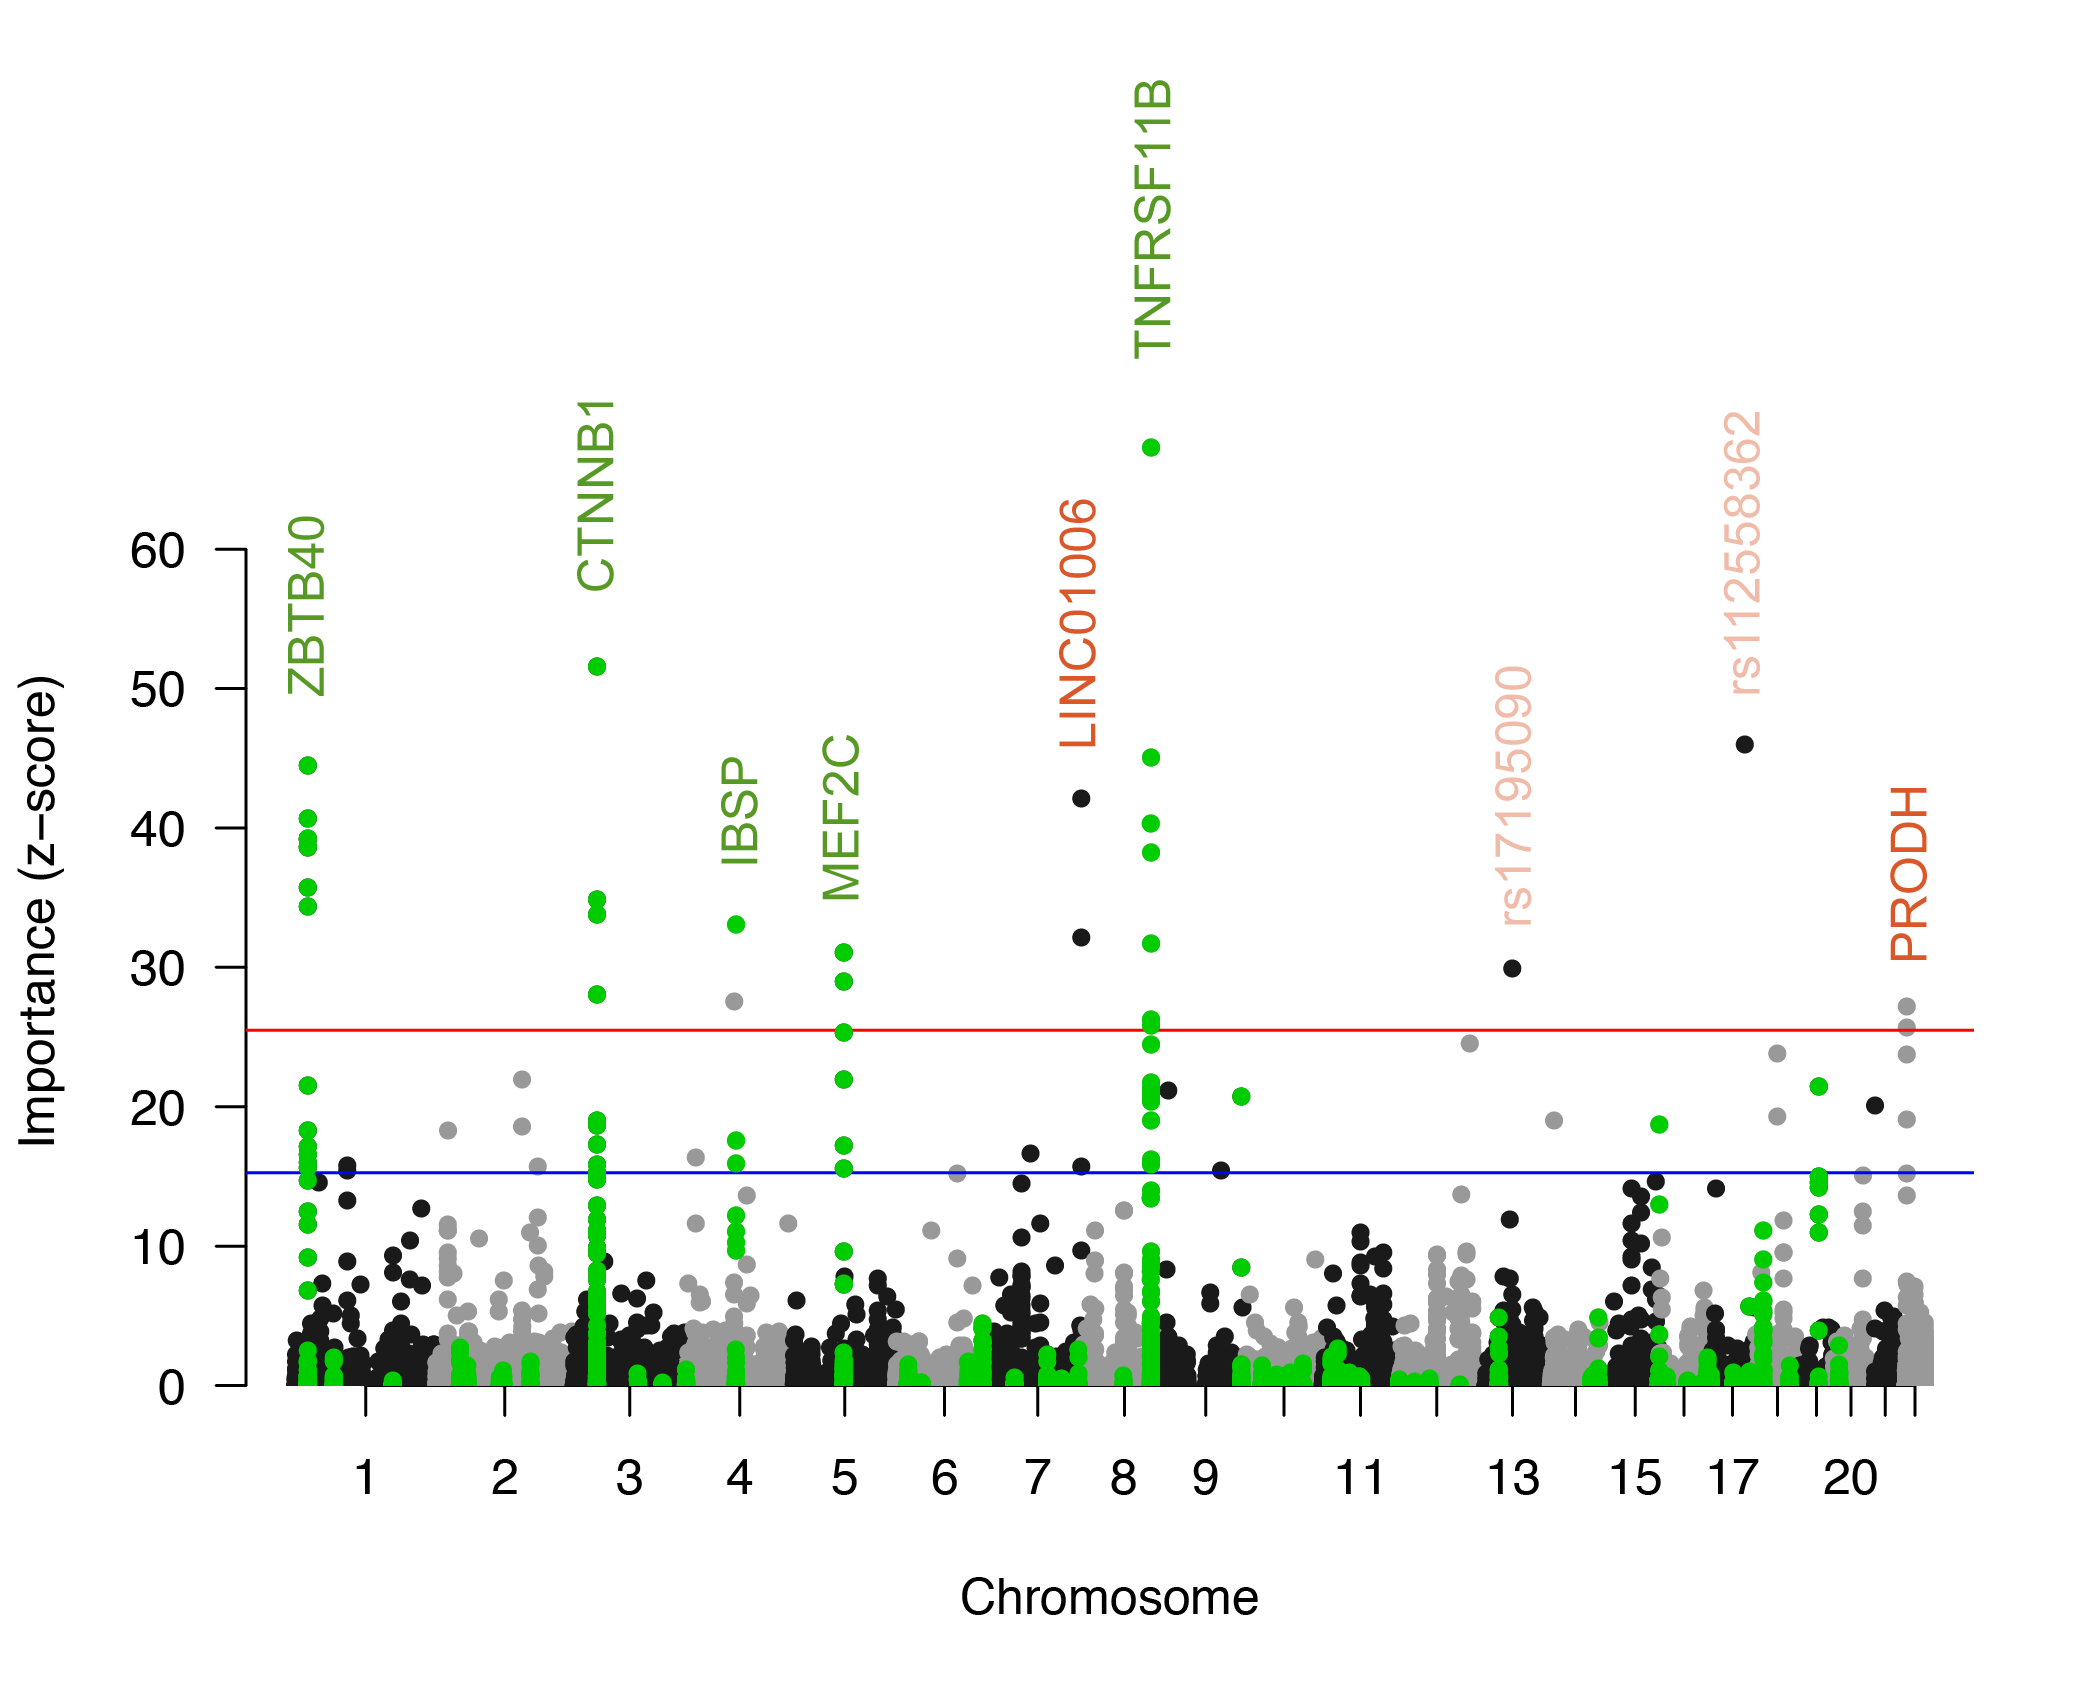
\includegraphics[totalheight=7cm]{./figs/BMDTopWholeGenome_annotated.png}
      \label{figure:BMDTopWholeGenome} 
    \end{subfigure} 
 \begin{subfigure}[b]{0.5\linewidth}
      \centering
      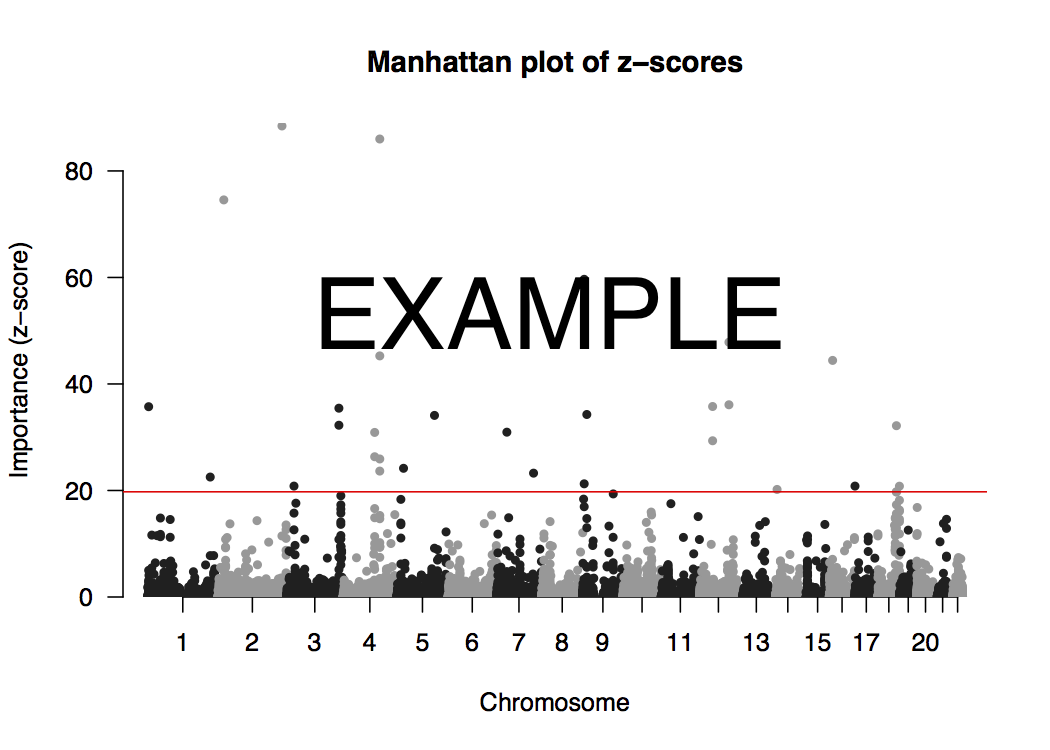
\includegraphics[totalheight=7cm]{./figs/BMDTopWholeGenome_BW_random.png}
      \label{zoomplotTNFRSF} 
   \end{subfigure} 
    \begin{subfigure}[b]{0.5\linewidth}
    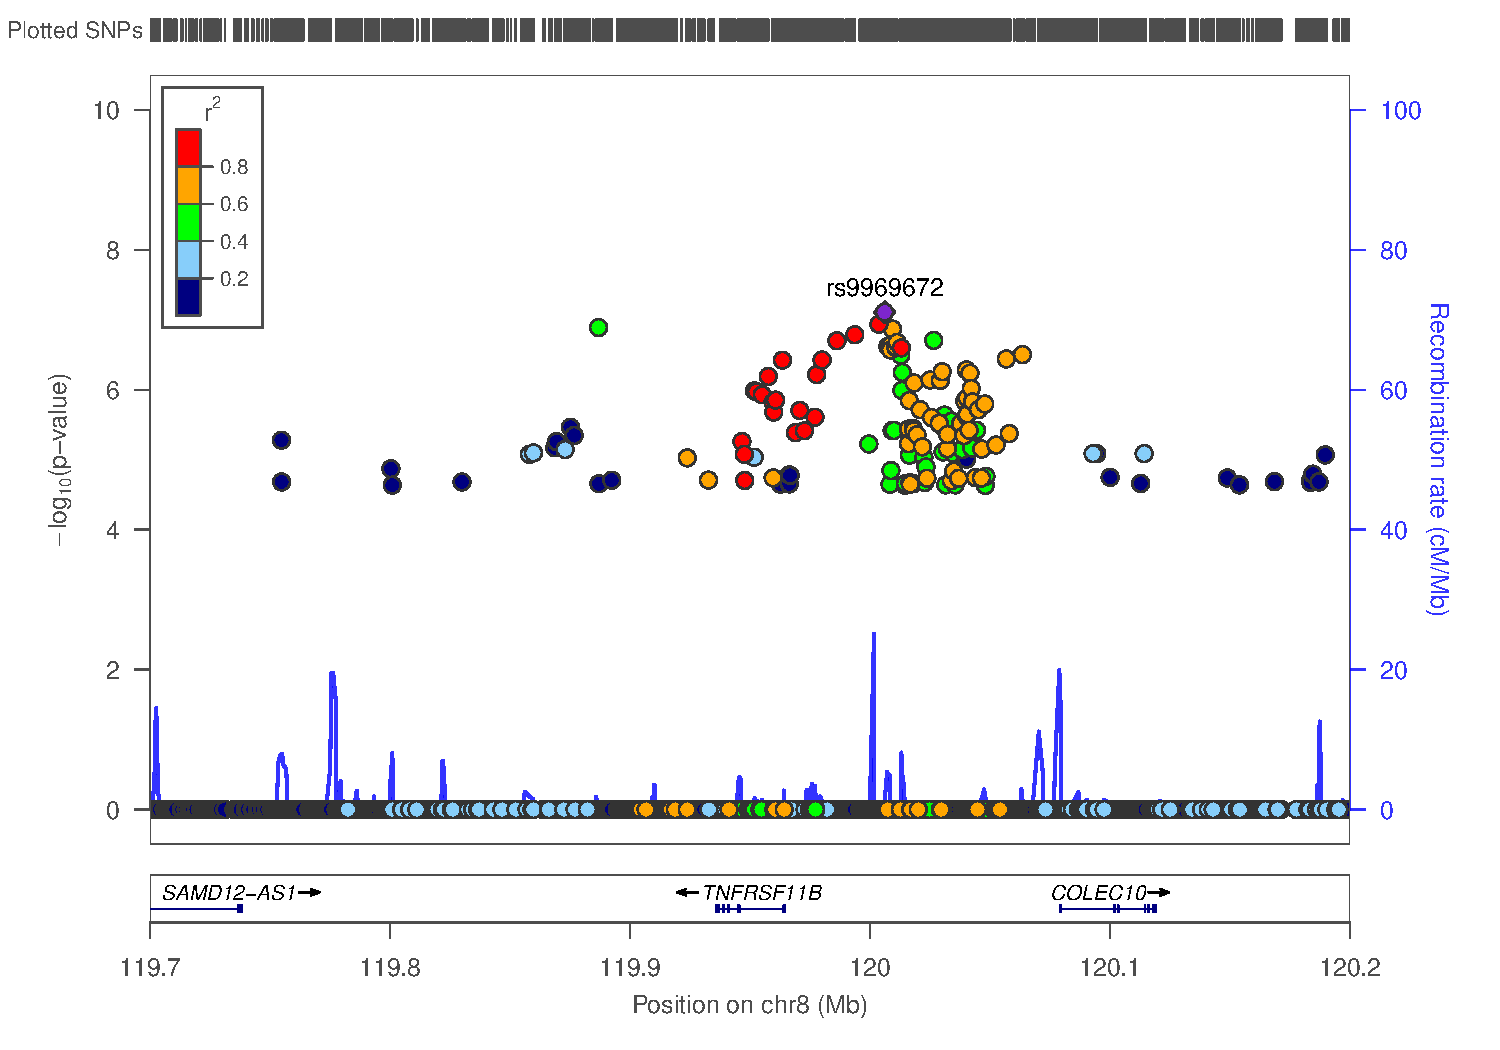
\includegraphics[totalheight=7cm]{./figs/new_10k_TNFRSF11B.pdf}
%     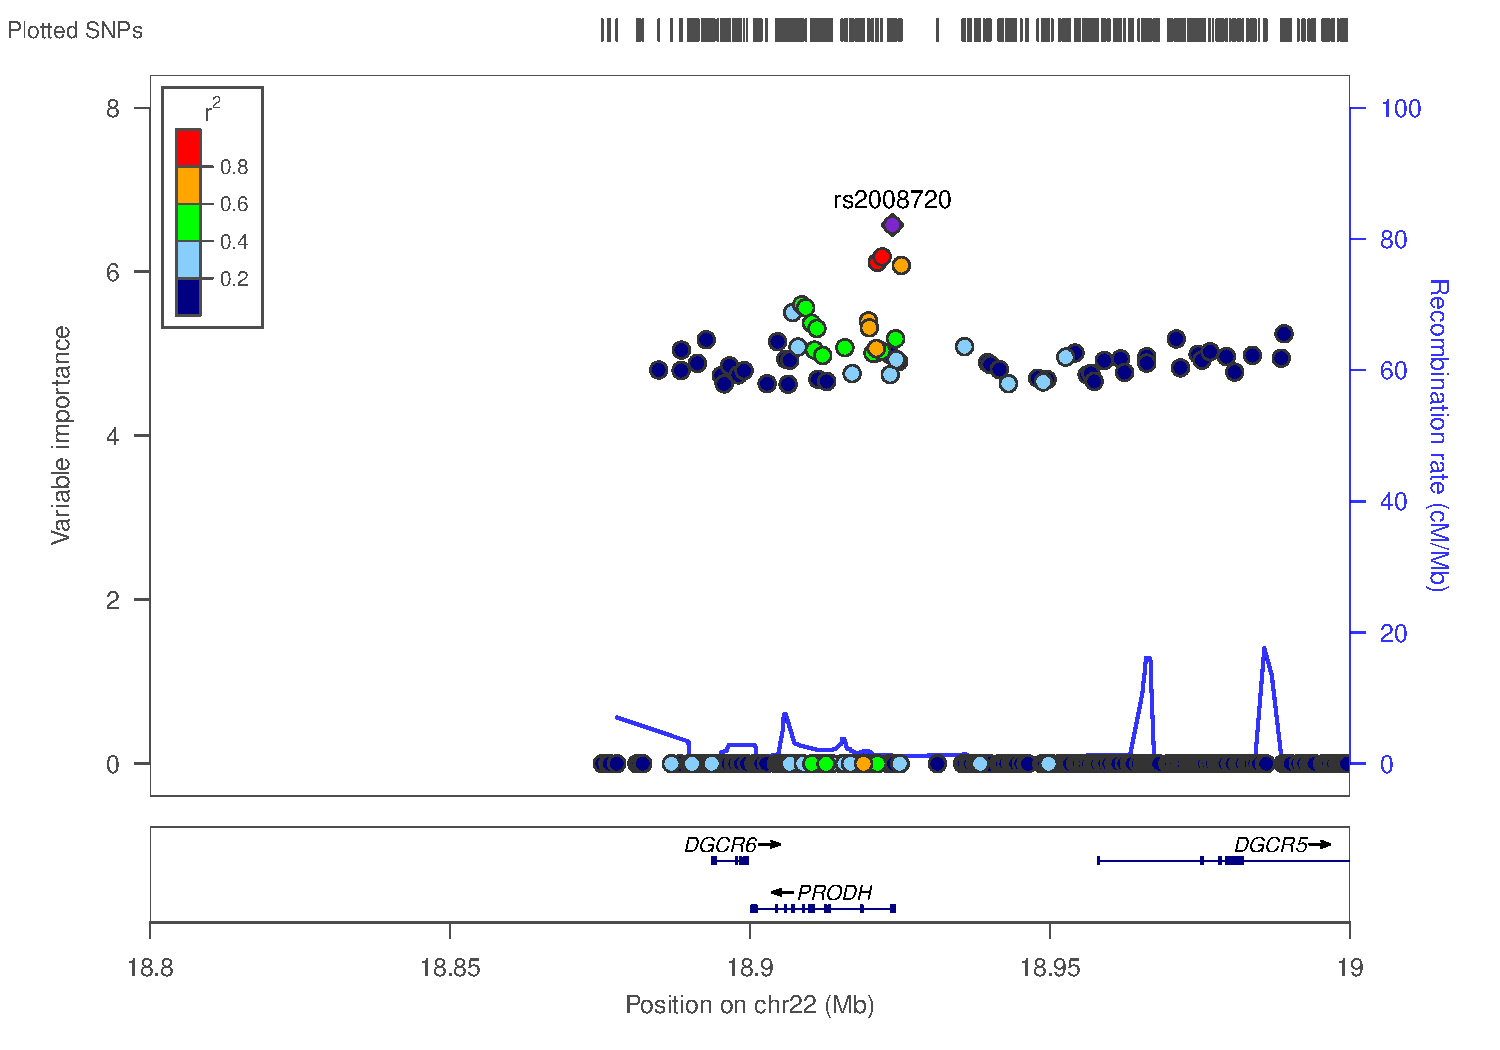
\includegraphics[totalheight=7cm]{./figs/new_10k_PRODH.pdf}
      \label{zoomplotprodh} 
    \end{subfigure} 
        \begin{subfigure}[b]{0.5\linewidth}
     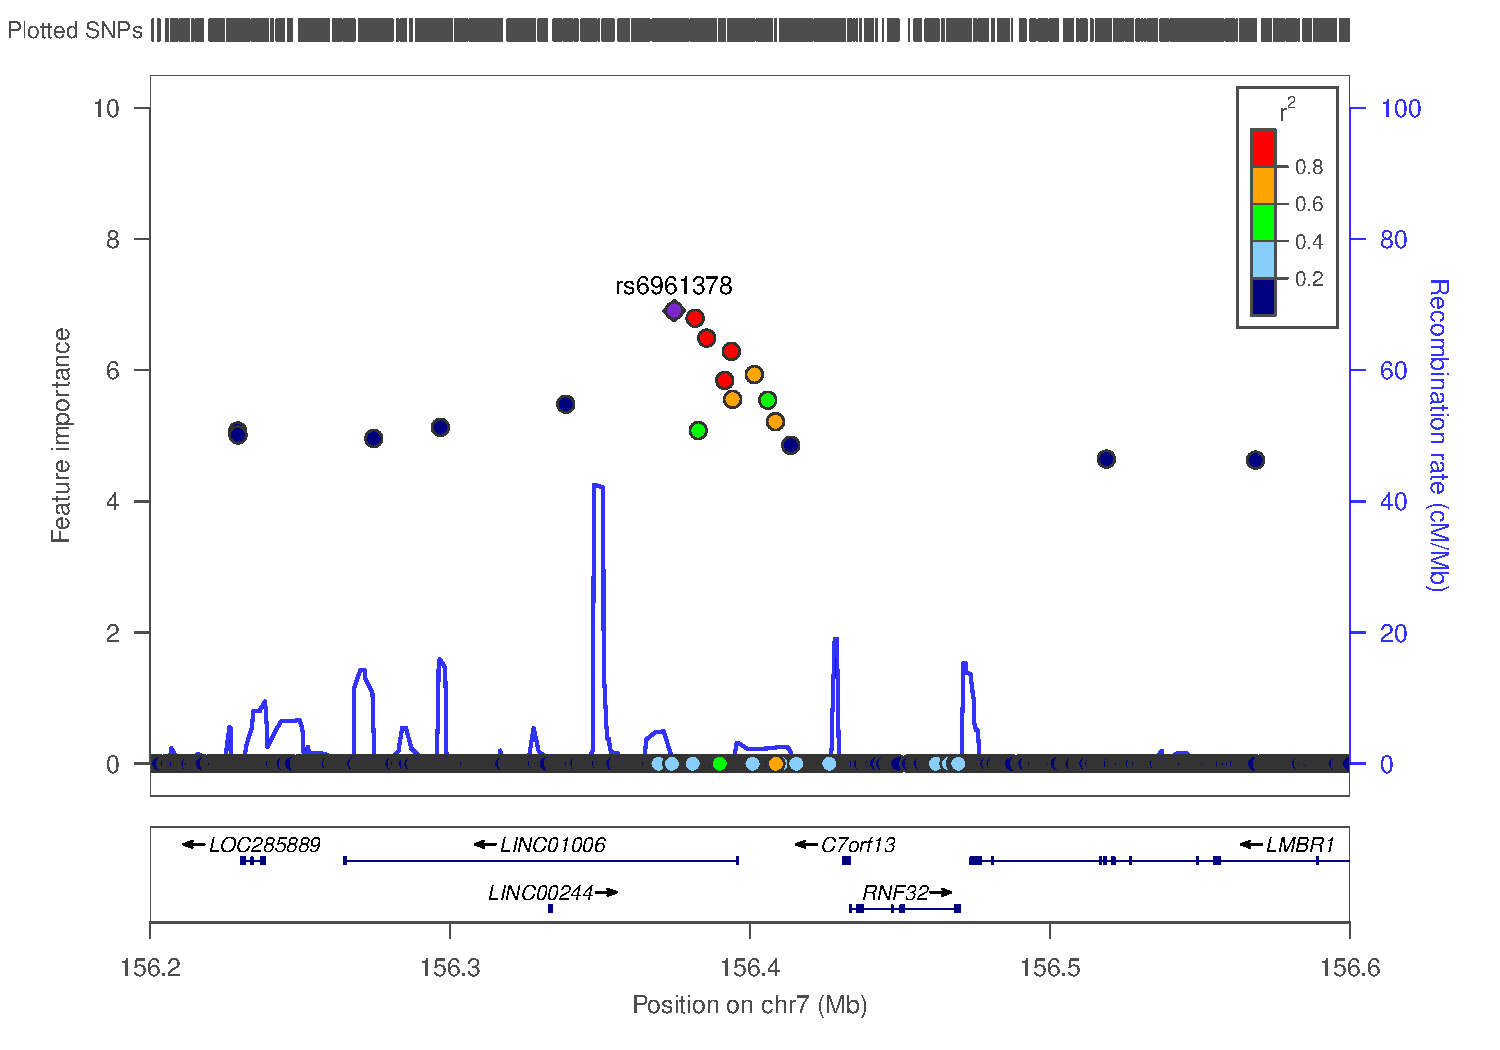
\includegraphics[totalheight=7cm]{./figs/EUR_chr7_156_2-156_6mb.pdf}
      \label{zoomplotlinc} 
    \end{subfigure} 
    \begin{flushleft}
      Genome-wide SNPs and their importance for the BMD dataset {\bf(a)}; highlighted are the 100 literature assigned BMD genes (green) and four novel loci. The horizontal line indicates the top 99.98 FDR. 
      {\bf(b)} shows a previous GWAS analysis using logistic regression. 
      Locus Zoomplot for {\bf(c)} the top ranked gene TNFRSF11B and the two putative novel associations {\bf(d)} LINC01006. Each point represents a variant with the normalised Gini impurity score on the left y axis and LD to the central SNP in colour with the highest $r^2$ in red.
     \end{flushleft}
  \end{adjustwidth}
        \label{manhattenzoom} 
\end{figure}


%\begin{figure}[tbhp]
%  \begin{adjustwidth}{-2.00in}{0in}
%    \caption{\textbf{Importance of 10,000 top ranked features and visualisation of the 22q.11 region}}
%    \label{figure:ranksumtest}
%     \begin{subfigure}[b]{0.5\linewidth}
%    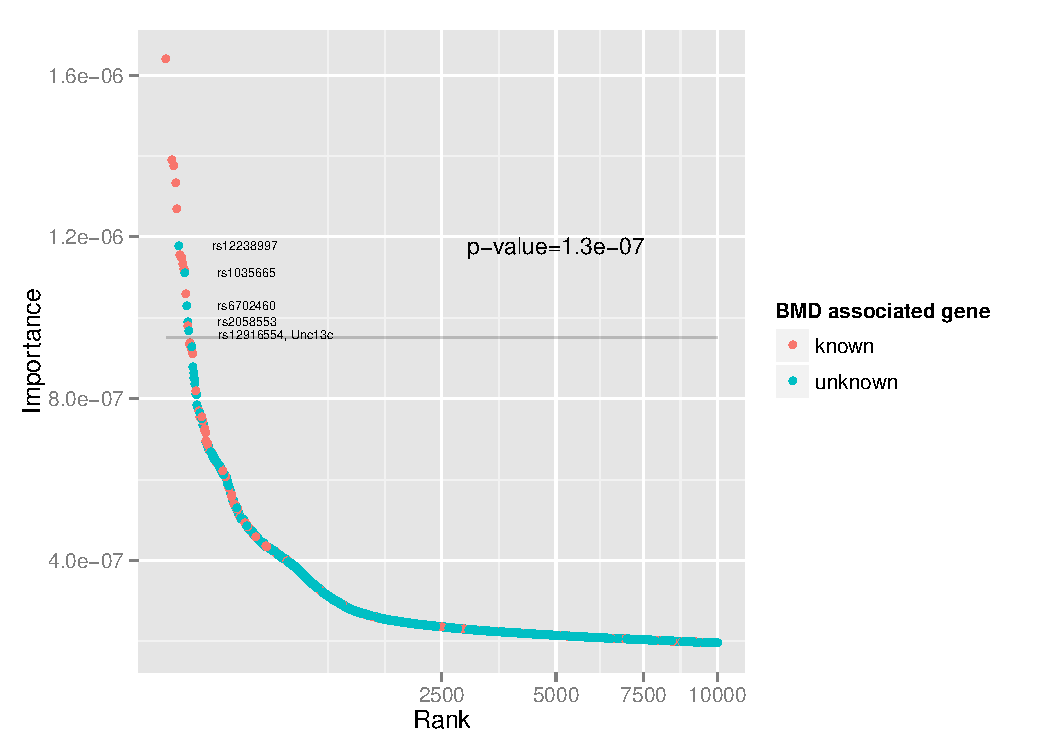
\includegraphics[totalheight=7cm]{./figs/BMDTop10K.pdf}
%     \caption{Distribution of known BMD genes amongst the top 10,000 features.} 
%      \label{figure:rbo-prod.png} 
%%      \vspace{4ex}
%    \end{subfigure} 
% \begin{subfigure}[b]{0.5\linewidth}
%      \centering
%      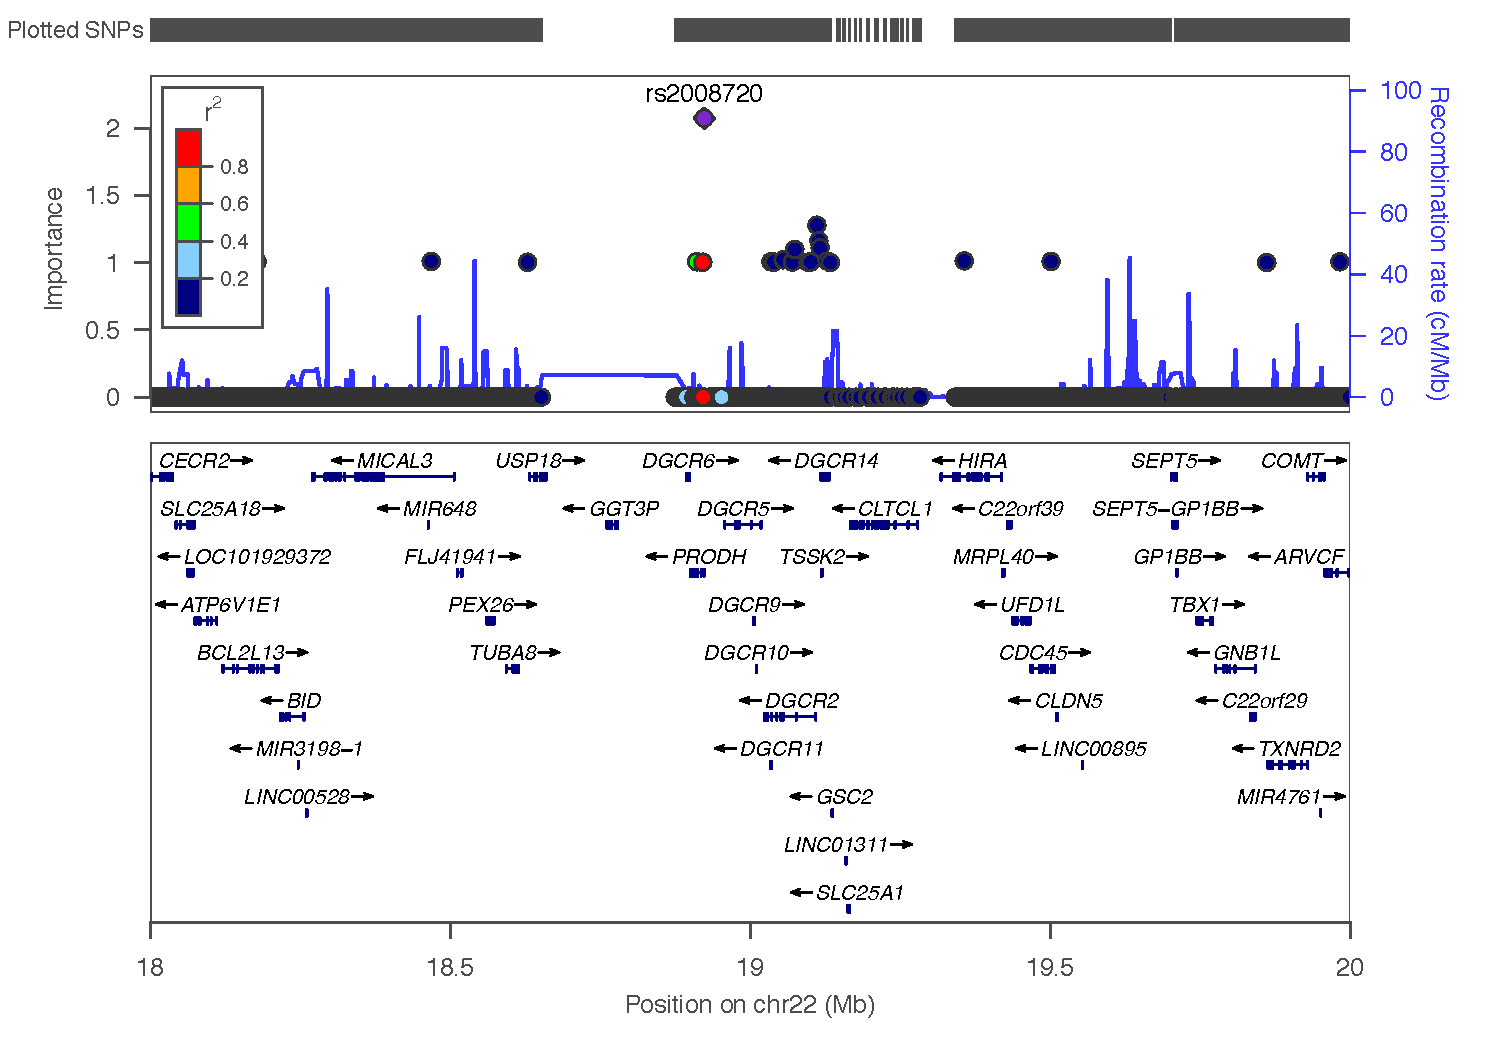
\includegraphics[totalheight=7cm]{./figs/EURchr22_18-20mb.pdf}
%      \caption{Zoom plot of the 22q.11 region centred on PRODH.} 
%      \label{zoomplot} 
%%      \vspace{4ex}
%    \end{subfigure} 
%    \begin{flushleft}
%      (a) The figure shows the top 10,000 features by their rank and Gini impurity score (Importance). The line denotes
%      the top 20 features which contains five novel loci annotated with text. The $p$-value is the Mann-Whitney U test.
%      (b) Each point represents a variant with the normalised Gini impurity score on the left y axis and LD in colour
%      with the highest $r^2$ in red.
%     \end{flushleft}
%  \end{adjustwidth}
%\end{figure}


%\begin{figure}[tbhp]
%  \begin{adjustwidth}{-2.00in}{0in}
%    \caption{\textbf{Importance of genome-wide SNPs}}
%    \label{figure:knowngeneranks}
%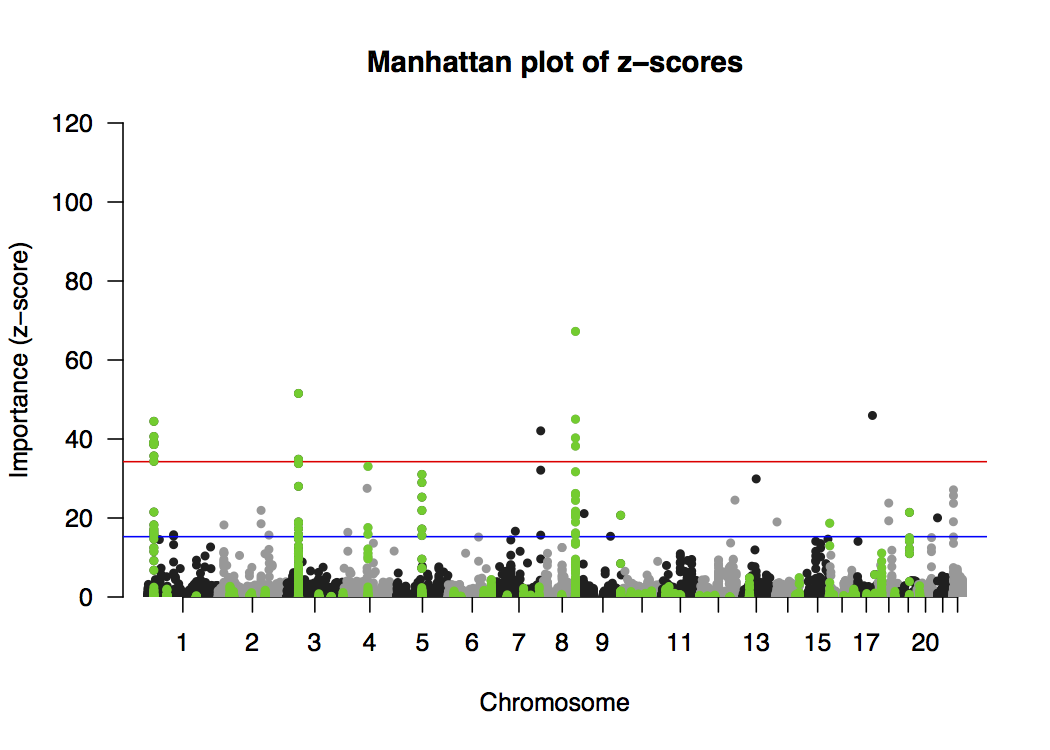
\includegraphics[totalheight=6.5cm]{./figs/BMDTopWholeGenome.pdf}
%    \begin{flushleft}
%      The figure shows genome-wide SNPs and their importance. Highlighted are the 100 literature assigned BMD genes. The horizontal line indicates the top 20. 
%     \end{flushleft}
%  \end{adjustwidth}
%\end{figure}



%1:693731 rs12238997 lncRNA
% rs1035665 A genome-wide association study of global gene expression http://www.nature.com/ng/journal/v39/n10/full/ng2109.html rs1035665 as master regulator of ATP Binding Cassette Subfamily F Member 2 ABCF1  with ABCF2 634 known 
% rs6702460 1	91536	91536	14	1.0296212827525244E-6 ncRNA
% rs2058553 2	20573002	20573002	15	9.896033178354981E-7 ncRNA
% rs12916554 15	 54607255	54607255	17	9.687391928109767E-7  Unc13c quality of sleep http://www.nature.com/ng/journal/v48/n8/full/ng.3595.html   https://www.ncbi.nlm.nih.gov/pubmed/27655463



%%%%%%%%%%%%%%%%%%%%%%%%%%%%%%%%
% Section 3: Classification selection
%%%%%%%%%%%%%%%%%%%%%%%%%%%%%%%%
\subsection{\cursedforest outperforms existing methods for classification problems}
In this section we demonstrate \cursedforest's classification accuracy on biological data and compare its performance against other published methods. 
We do this by predicting the ethnicity of the individuals in the 1000 Genomes Project from their genomic profiles and evaluate against the annotated label. 
We record the prediction error (OOB) as well as the runtime for each method. 
%@Aidan is 12 correct?
We limit the number of executors to 12 that are available to \cursedforest\ to keep the comparison fair for all methods.  

As shown in Fig.~\ref{figure:1000genomes}, only \cursedforest\ is able to scale to the full phase3\_chr1-22 dataset (2,504 samples x 19,328,051 variants), with
the standard random forest implementation in R running out of resources on the relatively low-dimensional
phase1\_chr22 dataset (1,092 x 490,036). 
Ranger's c++ implementation and the R front-end version of it are able to process the second largest dataset (phase3\_chr1-3 with 2,504 x 19,328,051), however, both are unable to process larger datasets successfully. 
While the c++ implementation runs out of memory the R front-end, which also covers the loading and pre-processing, needs an unreasonable compute time for this task (>20h), see Supplementary Table 1.
The standard implementation of random forest in SparkML already runs out of memory after processing the third largest dataset, phase3\_chr1 (2,504 x 6,450,364). 
This demonstrates that Spark ML, although designed to handle many samples, is unable to efficiently cope with large numbers of features. 

All tested methods have a worse runtime than \cursedforest\ for the datasets they processed successfully, except for the smallest dataset where the overhead of Spark's distributed platform made ranger's R implementation faster with 1 min 10 seconds compared to 1 min 50 seconds. For example, on phase3\_chr1-3 \cursedforest\ finishes in 1 hour, with ranger(R) requiring 4 hours and SparkML already needing 8 hours on a smaller dataset. 
Extrapolating from this, all comparable implementations hence would require more than 24 hours to finish, assuming the use of larger memory nodes.  

As our implementation can efficiently utilise large numbers of commodity nodes, the performance of \cursedforest\ can be substantially improved further. 
%@Aidan is 130 correct?
Table~\ref{cursedforesttable} shows the runtime when utilising the full Spark cluster (130 worker nodes). 

Building a model with \cursedforest\ on phase3\_chr1, which previously took 20 minutes, can be reduced to 4 minutes. 
Subsequently, phase3\_chr1-3 takes about 11 minutes, and building a
model on the entire genome is 37 minutes. 

Not only does the job complete successfully using \cursedforest\, but building a random
forest model on all 22 autosomes (phase3\_chr1-22)  leads to a more accurate result. 
The error can be reduced from OOB=0.04 when using only data from Chr1, which represents processing power limit for most tools, down to OOB=0.01 when using the full dataset. 


\begin{table}[!ht]
\begin{minipage}{\textwidth}
\centering
\caption{ {\bf Performance comparison with \cursedforest on different subsets of the 1000 Genomes Project data.}}
\begin{tabular}{| l | r | l |}
\hline
{\bf Genome \%} & {\bf Error} & {\bf Runtime} \\ \thickhline
phase1\_chr22: 1,092 x 490,036 & 0.04 & 1 min 5 seconds \\ \hline
phase3\_chr22: 2,504 x 1,103,548 & 0.06 & 1 min 37 seconds \\ \hline
phase3\_chr1: 2,504 x 6,450,364 & 0.04 & 4 min 10 seconds \\ \hline
phase3\_chr1-3: 2,504 x 19,328,051 & 0.02 & 10 min 49 seconds \\ \hline
phase3\_chr1-22: 2,504 x 81,047,467 & 0.01 & 36 min 54 seconds \\ \hline
\end{tabular}
\begin{flushleft} 
Comparison of runtime and error for models built using \cursedforest on different subsets of variant data 
from the 1000 Genomes Project.
Each random forest model consists of 50 trees and was built using 130 worker nodes, each with 8GB RAM.
\end{flushleft}
\label{cursedforesttable}
\end{minipage}
\end{table}


\begin{figure}[tbhp]
  \begin{adjustwidth}{-1.00in}{0in}
    \caption{\textbf{Runtime comparison on the 1000 genomes project}}
    \label{figure:1000genomes}
    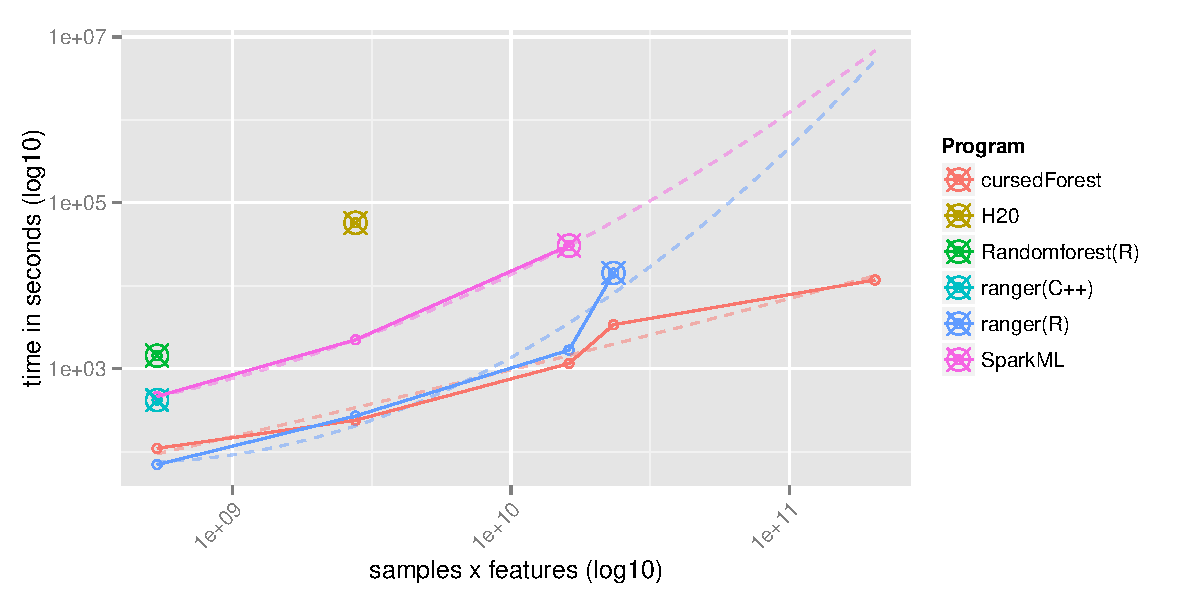
\includegraphics[totalheight=8cm]{./figs/1000genomesRuntime.pdf}
    \begin{flushleft}
      The figure shows the runtime for the 5 subsets of the 1000 genomes project and the different methods investigated.
      $\bigotimes$ marks the last dataset the different method completed before running out of memory or running more than
      20 hours. The dashed lines mark the trajectory for how \ranger and Spark ML had performed given larger memory machines.
    \end{flushleft}
  \end{adjustwidth}
\end{figure}




%%%%%%%%%%%%%%%%%%%%%%%%%%%%%%%%%
%% Section 1:  Feature Selection and classification on synthetic data
%%%%%%%%%%%%%%%%%%%%%%%%%%%%%%%%%
\subsection{\cursedforest can evaluate variable importance and perform classification for millions of features}
%\label{section:synthetic}
In this section we test the limits of \cursedforest\'s association testing and classify ability on high-dimensional data. 
%In this section we demonstrate the two features of \cursedforest, namely: variable selection analysis to select the most
%associated set of features amongst millions of dimensions; and its ability to accurately classify the labels of
%high-dimensional samples.  
We therefore generate a synthetic dataset with 2.5 million variables ($p=2,500,000$), of which 5 
are related to the response variable, and 5000 samples ($n=5000$), as discussed in the methods section.

We fit the random forest model and estimate the classification accuracy by capturing the out-of-bag error (OOB) and the
variable selection performance by capturing the rank-biased overlap (RBO) \cite{Webber2010} measure. RBO compares two
lists (in this case, the parameters $w_i, i=1,\ldots , 5$ (Equation~\ref{equation:synthetic.data}), and the top 1000
ranked variable importances from the \cursedforest model). It is a mesaure of similarity between rankings that handles
lists of different lengths, weighs high ranks more heavily than low, and is monotonic with increasing depth of
evaluation. We expect to retrieve the 5 features in order of the weight that was assigned to them and with a higher
variable importance measure than the noise variables. RBO provides a quantiative measure of how close we come to this on
a scale from 0 (no feature recovered) to 1 (fully recovered). See supplementary information (S*) for more details.

We are running Apache Spark 1.6.1 on a YARN
cluster with 12 worker nodes each with 16 Intel Xeon E5-2660@2.20GHz CPU cores and 128 GB of RAM.

%mtry = number of variable seclection at each node - proportion of p 
%ntree= number of trees 

% mtry large makes trees correlated because the same important features have a higher chance of being selected
% overfitting because it picks random that happen to be 

As shown in Fig~\ref{figure:out-of-bag-prediction-error-prod.png} the default value for \mtry (number of variables
selected at each node) does not result in a good classification performance for this large feature dataset. Note that
the plot shows the proportion, $n/p,$ for \mtry\ with the default being $\sqrt{p} \approx 1581$ ($n/p=0.0006$).  The
OOB for this value of \mtry does not drop below 0.5, even when the number of trees are increased (\ntree).

Increasing \mtry\ in combination with \ntree\ yields the best performance with the OOB error essentially constant around 0.4
across a large range of of \mtry and \ntree values.  This is in contrast to the feature-selection performance, where the
RBO measure heavily depends on \ntree\ and gives better results with lower values of \mtry.

This may be because a large \mtry leads to more correlated trees as the same important features have a higher chance of
being selected in all, not yielding good performance outcomes.  This issue is less pronounced for classification error
where random features can mimic the response variable, hence resulting more in a performance plateau.  Increasing the
number of trees on the other hand improves performance especially when the trees are kept diverse (small \mtry) but
appropriate for large feature datasets (\mtry larger than default). \cursedforest's feature of parallelizing trees at
the node level hence caters perfectly to the requirement of large feature datasets as more trees can be built given a
fixed time budget.

%Fig~\ref{figure:synth1} illustrates the effect of varying \mtry and \ntree on these two measures. The default \mtry
%value for a classification problem is $\sqrt{p} \approx 1581$ so in this case we are considering values considerably larger than
%the default. Fig~\ref{figure:out-of-bag-prediction-error-prod.png} shows the OOB error is constant across a large range of 
%of \mtry and \ntree values whereas Fig~\ref{figure:rbo-prod.png} illustrates that the RBO measure depends
%heavily on \ntree but gives a better value with lower values of \mtry.

From the synthetic data we can conclude that \cursedforest is able to perform accurate feature selection as well as
accurate classification for large numbers of samples with large feature vectors.  We can also conclude that fine tuning
the model to accurately classify the dataset does not ensure good feature selection performance as there seems to be
little correspondence between the OOB and RBO measure.



\begin{figure}[tbhp] 
  \begin{adjustwidth}{-1.00in}{0in}
    \caption{\textbf{Out of bag classification error and rank-biased-overlap estimates}} 
    \label{figure:synth1}
    \begin{subfigure}[b]{0.5\linewidth}
      \centering
      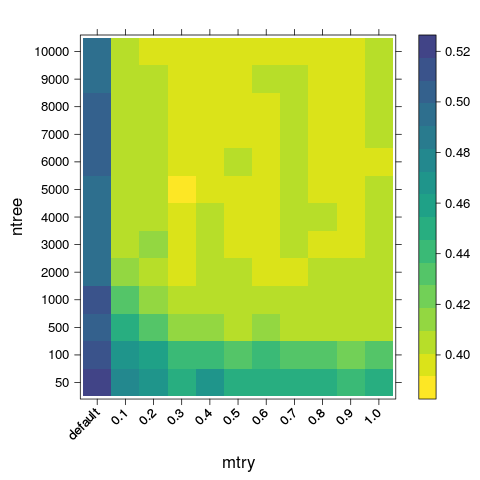
\includegraphics[totalheight=8cm]{./figs/oob_levleplot.png}
      \caption{OOB classification error.} 
      \label{figure:out-of-bag-prediction-error-prod.png} 
%      \vspace{4ex}
    \end{subfigure} 
    \begin{subfigure}[b]{0.5\linewidth}
      \centering
      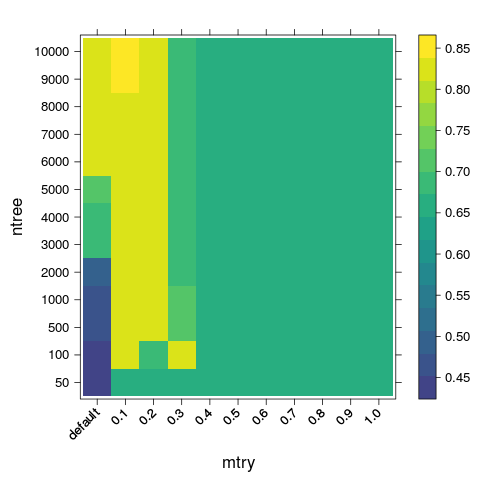
\includegraphics[totalheight=8cm]{./figs/rbo_levleplot.png}
      \caption{The rank-biased-overlap measure.} 
      \label{figure:rbo-prod.png} 
%      \vspace{4ex}
    \end{subfigure} 
    \begin{flushleft} 
      Random forests with 100 trees were trained on the synthetic dataset of 2.5M features and 5K samples.
      Each measure is shown as a function of \mtry and \ntree. Note that the plot colors have been chosen so that the lighter color indicates
      the better result, that is, a lower OOB or a higher RBO.
    \end{flushleft}
  \end{adjustwidth}
\end{figure}



%%%%%%%%%%%%%%%%%%%%%%%%%%%%%%%%
% Section 4: Sensitivity to different parameters and scalability
%%%%%%%%%%%%%%%%%%%%%%%%%%%%%%%%
\subsection{Scalability analysis}
In this section we explore the performance of \cursedforest\ in more detail by testing its ability to scale to different sizes of data
and computational resources.

In order to asses these characteristics, we run \cursedforest classification on synthetic datasets with varying numbers
of variables (features) and samples, similar to the dataset used in \cite{Wright.and.Ziegle.2016} to evaluate
\ranger, allocating varying number of CPU cores to the \cursedforest and also varying the computational complexity
of the random forests by using a range of \mtry values.

We investigate the different synthetic datasets generated for section \ref{section:synthetic_data} and measured the time
taken to build a random forest model of 100 trees. The results reported below are averages of 5 runs, and all the cases
were executed with the same random seed, to improve the consistency of measurements.

First we look at \cursedforest horizontal scalability for a medium size dataset of 2.5 million variables and 5000
samples, by varying the \mtry  fraction and the number of CPU cores allocated to the execution. 
%The results are visualised in Fig~\ref{figure:synthetictiming}. 
%The raw results are
%presented in Table~\ref{synthetictimingtable} and visualized in figure \ref{figure:synthetictiming} below. 
Regardless of the number of cores used, \cursedforest displays approximately linear dependency between the execution
time and \mtry (Fig~\ref{figure:synthetictiming.a}).

\cursedforest scales almost linearly with the number of CPU cores for medium values of \mtry fraction but for both lower
and higher values the performance degrades slightly (Fig~\ref{figure:synthetictiming.b}). In the latter case the likely
cause is communication overhead (with lower \mtry values the proportion of time for parallelizable computation to the
time for internode communication is lower) while in the latter case it is most likely caused by reaching the clusters
computational capacity.

Next we investigate \cursedforest scalability with regards to the size of data, by varying the number of variables and
sample for a fixed \mtry fraction of 0.25 and execution of 128 CPU cores. The results are visualized in
Fig~\ref{figure:synth2} below (please note log scale on the axes and the values on y axes are expressed as trees per
hour).

Generally, the number of trees per hour decreases with an increased number of variables and samples sizes. Some
irregularities in the graph can be attributed to computation vs communication tradeoff. It is also worth noting that
keeping the \mtry fraction constant results in higher \mtry values with the growing number of variables, and this is
what drives the performance down rather that the increase of dataset size itself.

To conclude \cursedforest is capable of processing 60 trees per hour on a datasets with 50 million variables and 10,000
samples, which is the size range for whole genome sequencing experiments of clinically relevant cohort sizes.

\begin{figure}[tbhp]
  \begin{adjustwidth}{-1.00in}{0in}
    \caption{\textbf{Scalability of the wide random forest on the synthetic dataset of 2.5M features and 5K samples.}}
    \label{figure:synthetictiming}
    \begin{subfigure}[b]{0.45\linewidth}
      \centering
      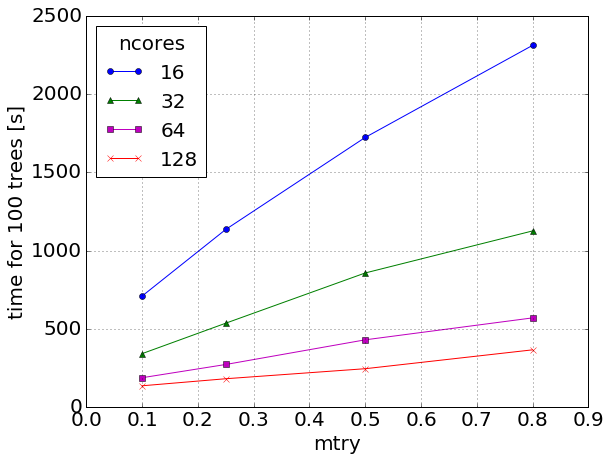
\includegraphics[totalheight=6cm]{./figs/mtry_cpu.png} 
      \caption{Time in seconds to build 100 trees for different \mtry\ fractions. } 
      \label{figure:synthetictiming.a} 
      \vspace{4ex}
    \end{subfigure} 
    \hfill
    \begin{subfigure}[b]{0.45\linewidth}
      \centering
      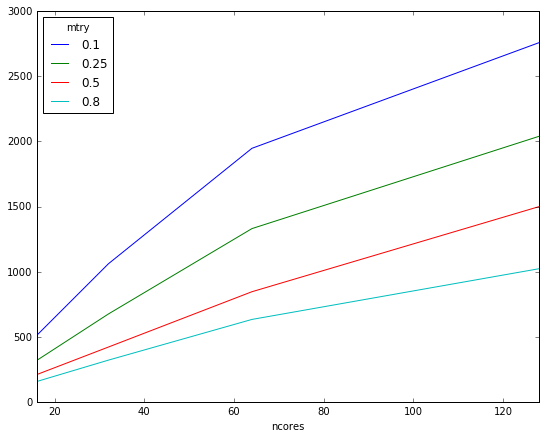
\includegraphics[totalheight=6cm]{./figs/cpu_mtry_trees_per_hour.png}
      \caption{Number of trees build per hour when using a growing number of CPU cores.}
      \label{figure:synthetictiming.b}
      \vspace{4ex}
    \end{subfigure} 
  \end{adjustwidth}
\end{figure}

% commented this table out -- see above
% \begin{table}[!ht]
%   \begin{adjustwidth}{-1.00in}{0in}
%     \centering
%     \caption{\textbf{
%  Time in seconds to build a random forest of 100
%   trees on 128 CPU cores with varying numbers of variables and samples.}}
% \label{synthetictimingtable}
% \begin{tabular}{|l|l|l|l|l|l|l|}
% \hline
% \multicolumn{2}{|l|}{\multirow{2}{*}{}}           & \multicolumn{5}{c|}{Number of variables} \\
% \cline{3-7}
% \multicolumn{2}{|l|}{}                               & \bf{150,000} & \bf{500,000} & \bf{2,500,000}  & \bf{10,000,000} & \bf{50,000,000} \\
% \hline                                                            
% \multirow{4}{*}{Number of samples}      & \bf{1000}  & 21.6  & 26.7  & 59.8  & 133.5  & 668.8 \\
%                                         & \bf{5000}  & 45.7  & 71.9  & 186.2 & 729.3  & 2887.4 \\
%                                         & \bf{10000} & 70.2  & 120.2 & 397.3 & 2237.8 & 5747.8 \\
% \hline
% \end{tabular}
% \end{adjustwidth}
% \end{table}



\begin{figure}[tbhp]
  \begin{adjustwidth}{-1.00in}{0in}
    \caption{\textbf{Scalablity of the Wide Random Forest on synthetic datasets with varying number of samples and variables.}}
    \label{figure:synth2}
    \begin{subfigure}[b]{0.5\linewidth}
      \centering
      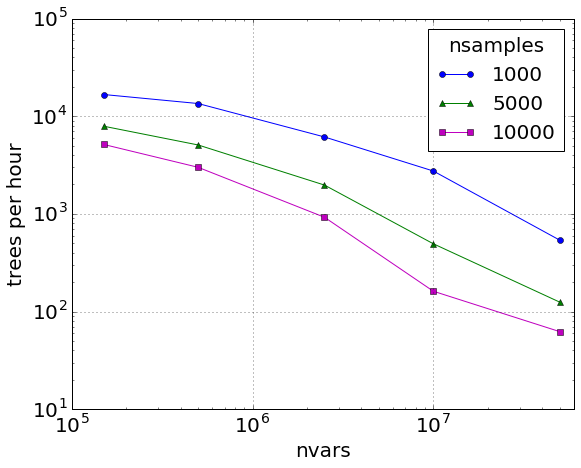
\includegraphics[totalheight=6cm]{./figs/nvars_nsamples.png} 
      \caption{Number of trees build per hour when growing number of variables.} 
      \label{figure:synth2.a} 
      \vspace{4ex}
    \end{subfigure} 
    \begin{subfigure}[b]{0.5\linewidth}
      \centering
      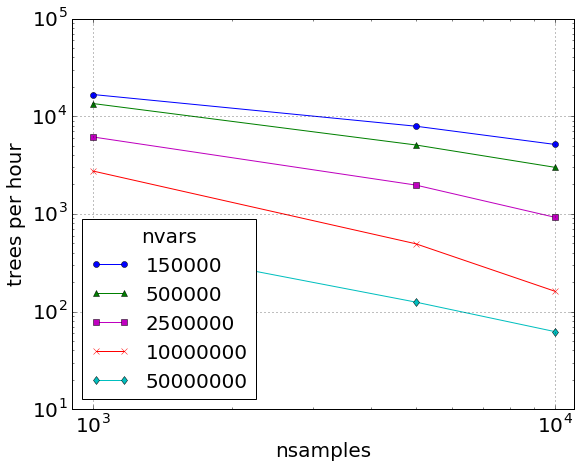
\includegraphics[totalheight=6cm]{./figs/nsamples_nvars.png}
      \caption{Number of trees build per hour when growing number of samples.}
    \label{figure:synth2.b}
    \vspace{4ex}
  \end{subfigure}
\end{adjustwidth}
\end{figure}

% no data in this table 
% \begin{table}[!ht]
% \caption{
% {\bf Sensitivity analysis on parameter choice.}}
% \begin{tabular}{|l|l|l|l|l|l|l|l|}
% \hline
% %\multicolumn{4}{|l|}{\bf Heading1} & \multicolumn{4}{|l|}{\bf Heading2}\\ \hline
% \bf{ \mtry\ }  & \bf{Mtree} & \bf{depth} & \bf{Accuracy} & \bf{Runtime} & \bf{Memory} \\
% \hline
% &&&&&\\ \hline
% \end{tabular}
% \begin{flushleft} 
%   Table notes here.
% \end{flushleft}
% \label{table2}
% \end{table}




\section{Conclusion}

Using a novel parallelization approach enabled by Spark, we extended random forests to cope with extremely high dimensional data (large number of variables). 
We have demonstrated that for datasets with more variable ($p$) than samples ($n$), such as GWAS applications, \cursedforest can perform effective variable selection replicating previous findings and uncovering novel associations in a Bone Mineral Density study. 
We are able to elevate the signal compared to previous approaches using logistic regression due to random forests also modelling interacting features.

In fact, \cursedforest's ability to almost exhaustively sample the combinatorial space by efficiently building large numbers of trees puts it closer than any other method to the theoretical boundary for accurate recovery of informative variables. Donoho and Tanner~\cite{Donoho.and.Tanner.2009} define this as the ``universal phase change'', which depends on underdetermination, $\delta = n/p$, and the sparsity, $\rho =k/n$ (where $k$ is the number of informative variables). 
By effectively operating in the difficult area of this space with $p >> n$ and small number of informative features, \cursedforest is pushing the practical limits of this paradigm. 

To showcase the breadth of application scope, we also demonstrate that \cursedforest's implementation aids in classification problems such as predicting the ethnicity of the 1000 genome project. 
By comparing \cursedforest\ to other implementations (including those optimised for large datasets) we have demonstrated that runtime can be improved by 80\% allowing analysis in timeframes relevant for point-of-care diagnostics such as for "Patients like mine" scenarios thereby enabling evidence based self learning health care. 

In summary, \cursedforest\  offers the broadly needed capability of performing sophisticated machine learning tasks on big, complex life science data. Specifically, the here demonstrated ability to uncover novel biological information from previously analysed GWAS studies showcases the enormous potential of re-analysing the GWAS catalogue given this unprecedented computational capacity to perform joint-loci association testing and identify the much-anticipated cumulative multi-gene disease contribution.    

%Donoho and Tanner \cite{Donoho.and.Tanner.2009} give a ``universal phase change'' result that has applications in a
%large number of areas, including variable selection in high dimensions. The theoretical phase change boundary is based on arguments
%from combinatorial geometry.
%
%They argue that there is a sharp disjunction between the cases where informative variables may be recovered with a high
%accuracy by procedures like stepwise variable selection, and the cases where they can not be recovered. The boundary is
%shown in Fig~\ref{figure:phase-diagram-equivalence.png} in a space parameterized by the level of underdetermination,
%$\delta = n/p$, and by the sparsity, $\rho =k/n$ (where $k$ is the number of informative variables).  Above the
%phase-transition line variable recovery is still possible by a combinatorial search approach such as all-subsets
%variable selection. 
%
%\begin{figure}[tbhp] 
% \begin{adjustwidth}{-1.00in}{0in}
%    \centering
%    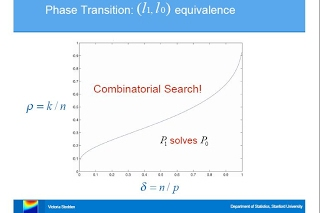
\includegraphics[totalheight=6cm]{./figs/phase-diagram-equivalence.png} 
%    \caption{{\bf The phase change diagram.}}
%    \label{figure:phase-diagram-equivalence.png} 
%    \vspace{4ex}
%  \end{adjustwidth}
%\end{figure}
%
%
%\cite{Donoho.and.Stodden.2006} investigate the phase transition in a small simulation.  They consider a regression
%problem with $\underset{n\times p}{X}\sim N(0,1)$ with $p$ fixed at 200 and $n$ variable.  They set
%$\beta(1:k) \sim U(1,100)$ and $\beta((k+1):p) =0$, then $y= X\beta + \epsilon$ with $\epsilon \sim N(0,\sqrt{16})$. They
%evaluate variable selection by the error measure
%$$\frac{\Vert\hat{\beta}-\beta\Vert_2}{\Vert\beta\Vert_2}.$$
%
%They consider a number of variable selection methods, including a false discovery rate criteria. This involves adding
%the variable with the maximum $t$-value to the linear model if the $p$-value is less than 
%$0.25(\text{number of  terms  currently  in  the  model})/(\text{total  number  of  variables})$.  
%See Fig~\ref{figure:error_Stodden_FDR.png} for the error measure and
%figure \ref{figure:rbo_Stodden_FDR.png} for the RBO, comparing the ranking (i.e. values) of $\hat{\beta}$ and $\beta$.
%It apparent that there is a marked drop in the accuracy of the variable recovery in line with the prediction of the
%Donoho-Tanner phase transition.
%
%
%
% \begin{figure}[tbhp] 
%%   \begin{adjustwidth}{-1.00in}{0in}
%     \begin{subfigure}[t]{0.5\linewidth}
%       \centering
%       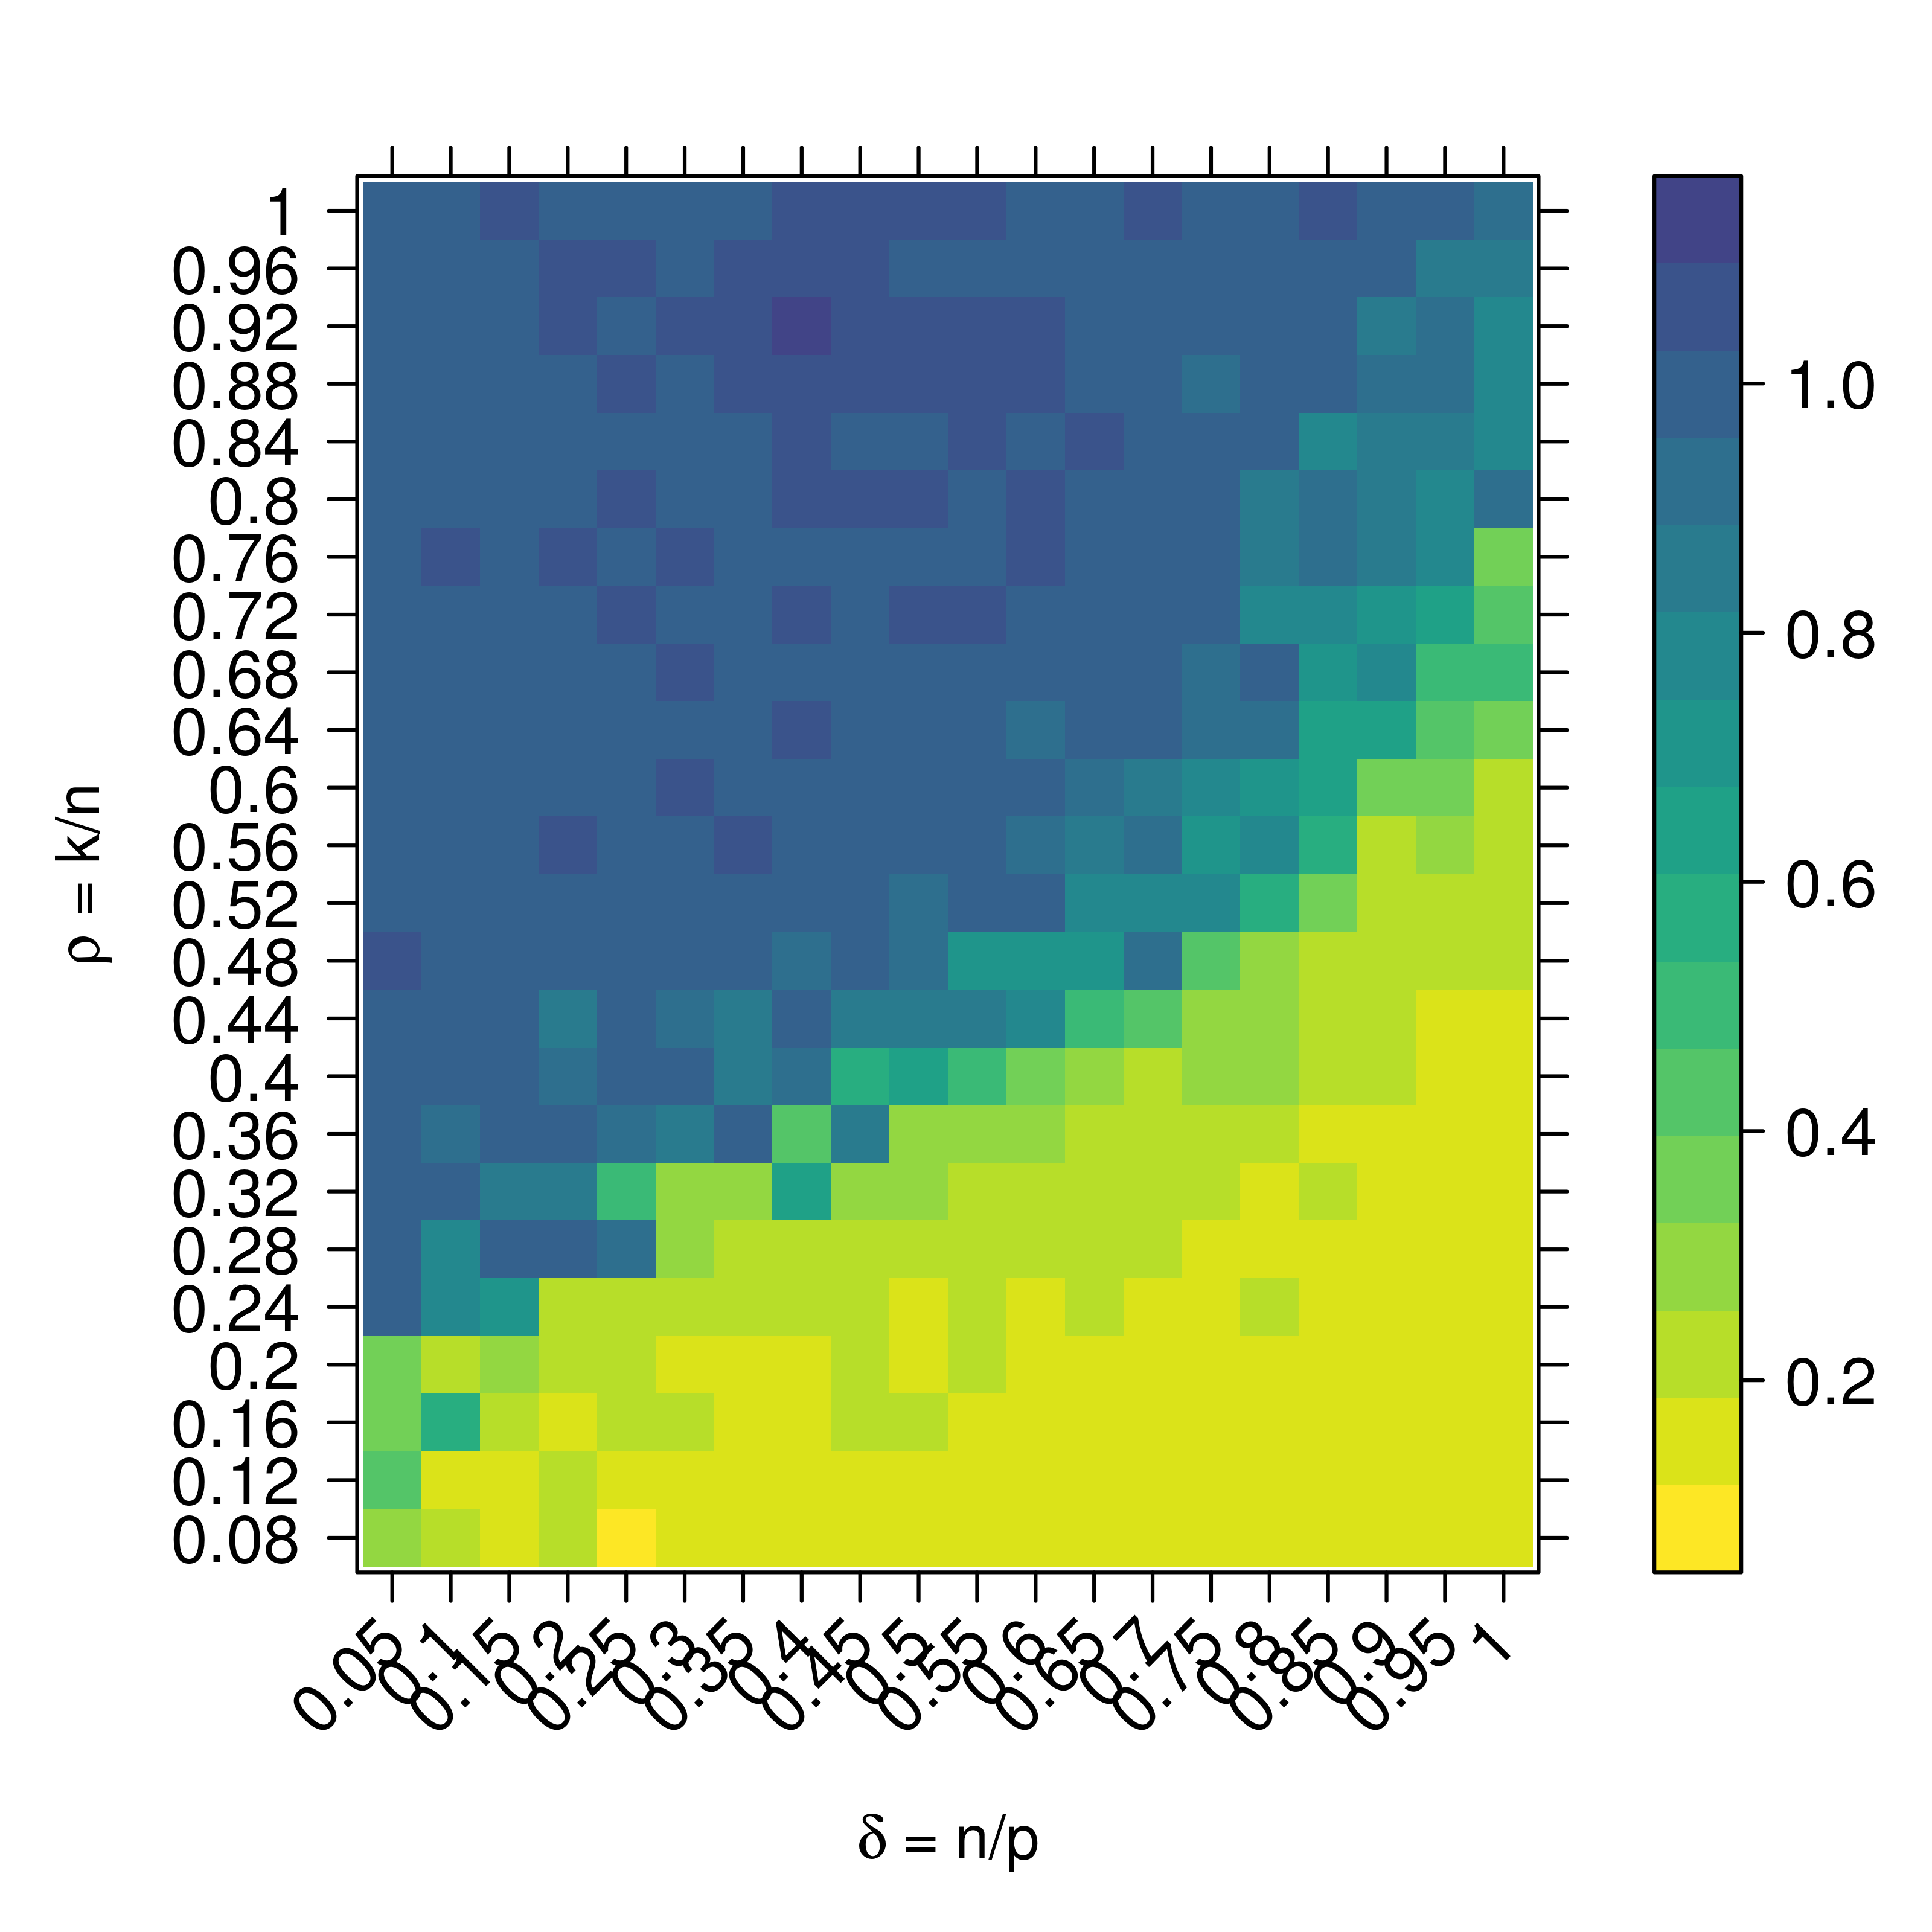
\includegraphics[totalheight=6cm]{./figs/error_Stodden_FDR.png}
%       \caption{The error measure.}
%       \label{figure:error_Stodden_FDR.png}
%%       \vspace{4ex}
%     \end{subfigure} 
%     \begin{subfigure}[t]{0.5\linewidth}
%       \centering
%       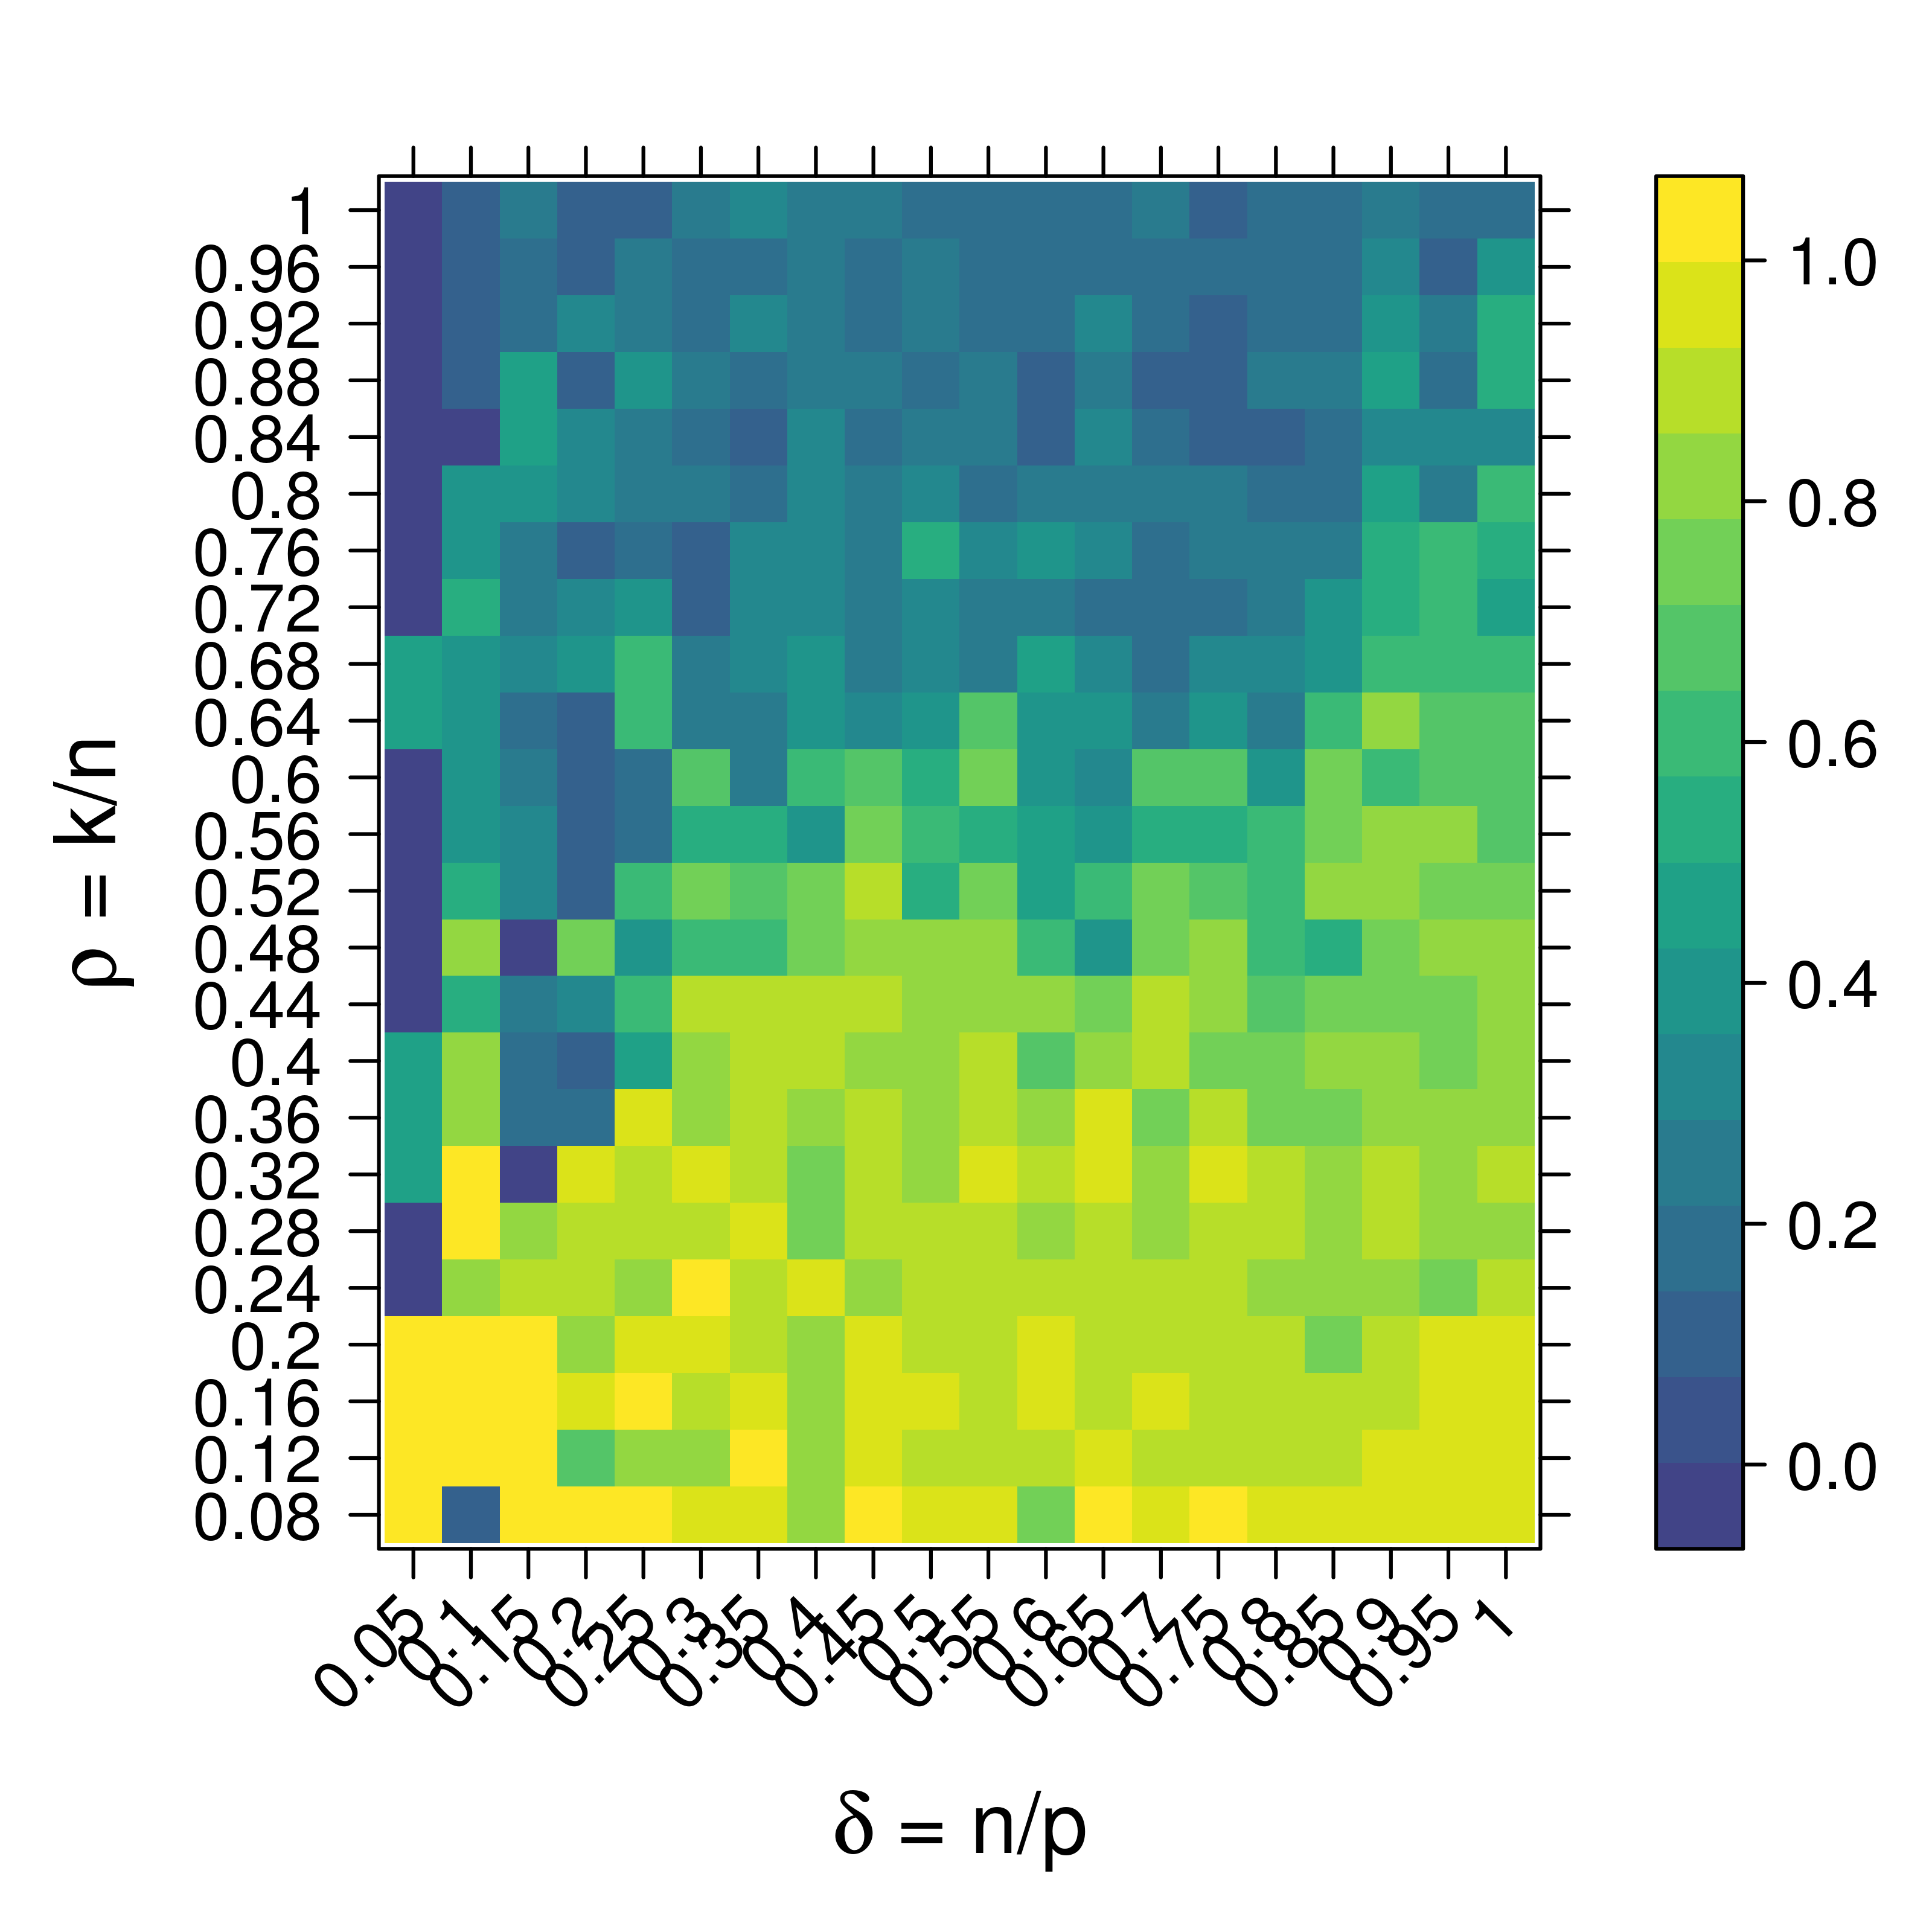
\includegraphics[totalheight=6cm]{./figs/rbo_Stodden_FDR.png}
%       \caption{The RBO measure}
%       \label{figure:rbo_Stodden_FDR.png}
%     \end{subfigure} 
%     \caption{Forward stepwise variable selection with a false discovery rate stopping criteria.}
%       \label{figure:error_and_rbo_Stodden_FDR.png}
%%   \end{adjustwidth}
% \end{figure}
%
% \begin{figure}[tbhp] 
%%   \begin{adjustwidth}{-1.00in}{0in}
%     \begin{subfigure}[t]{0.5\linewidth}
%       \centering
%       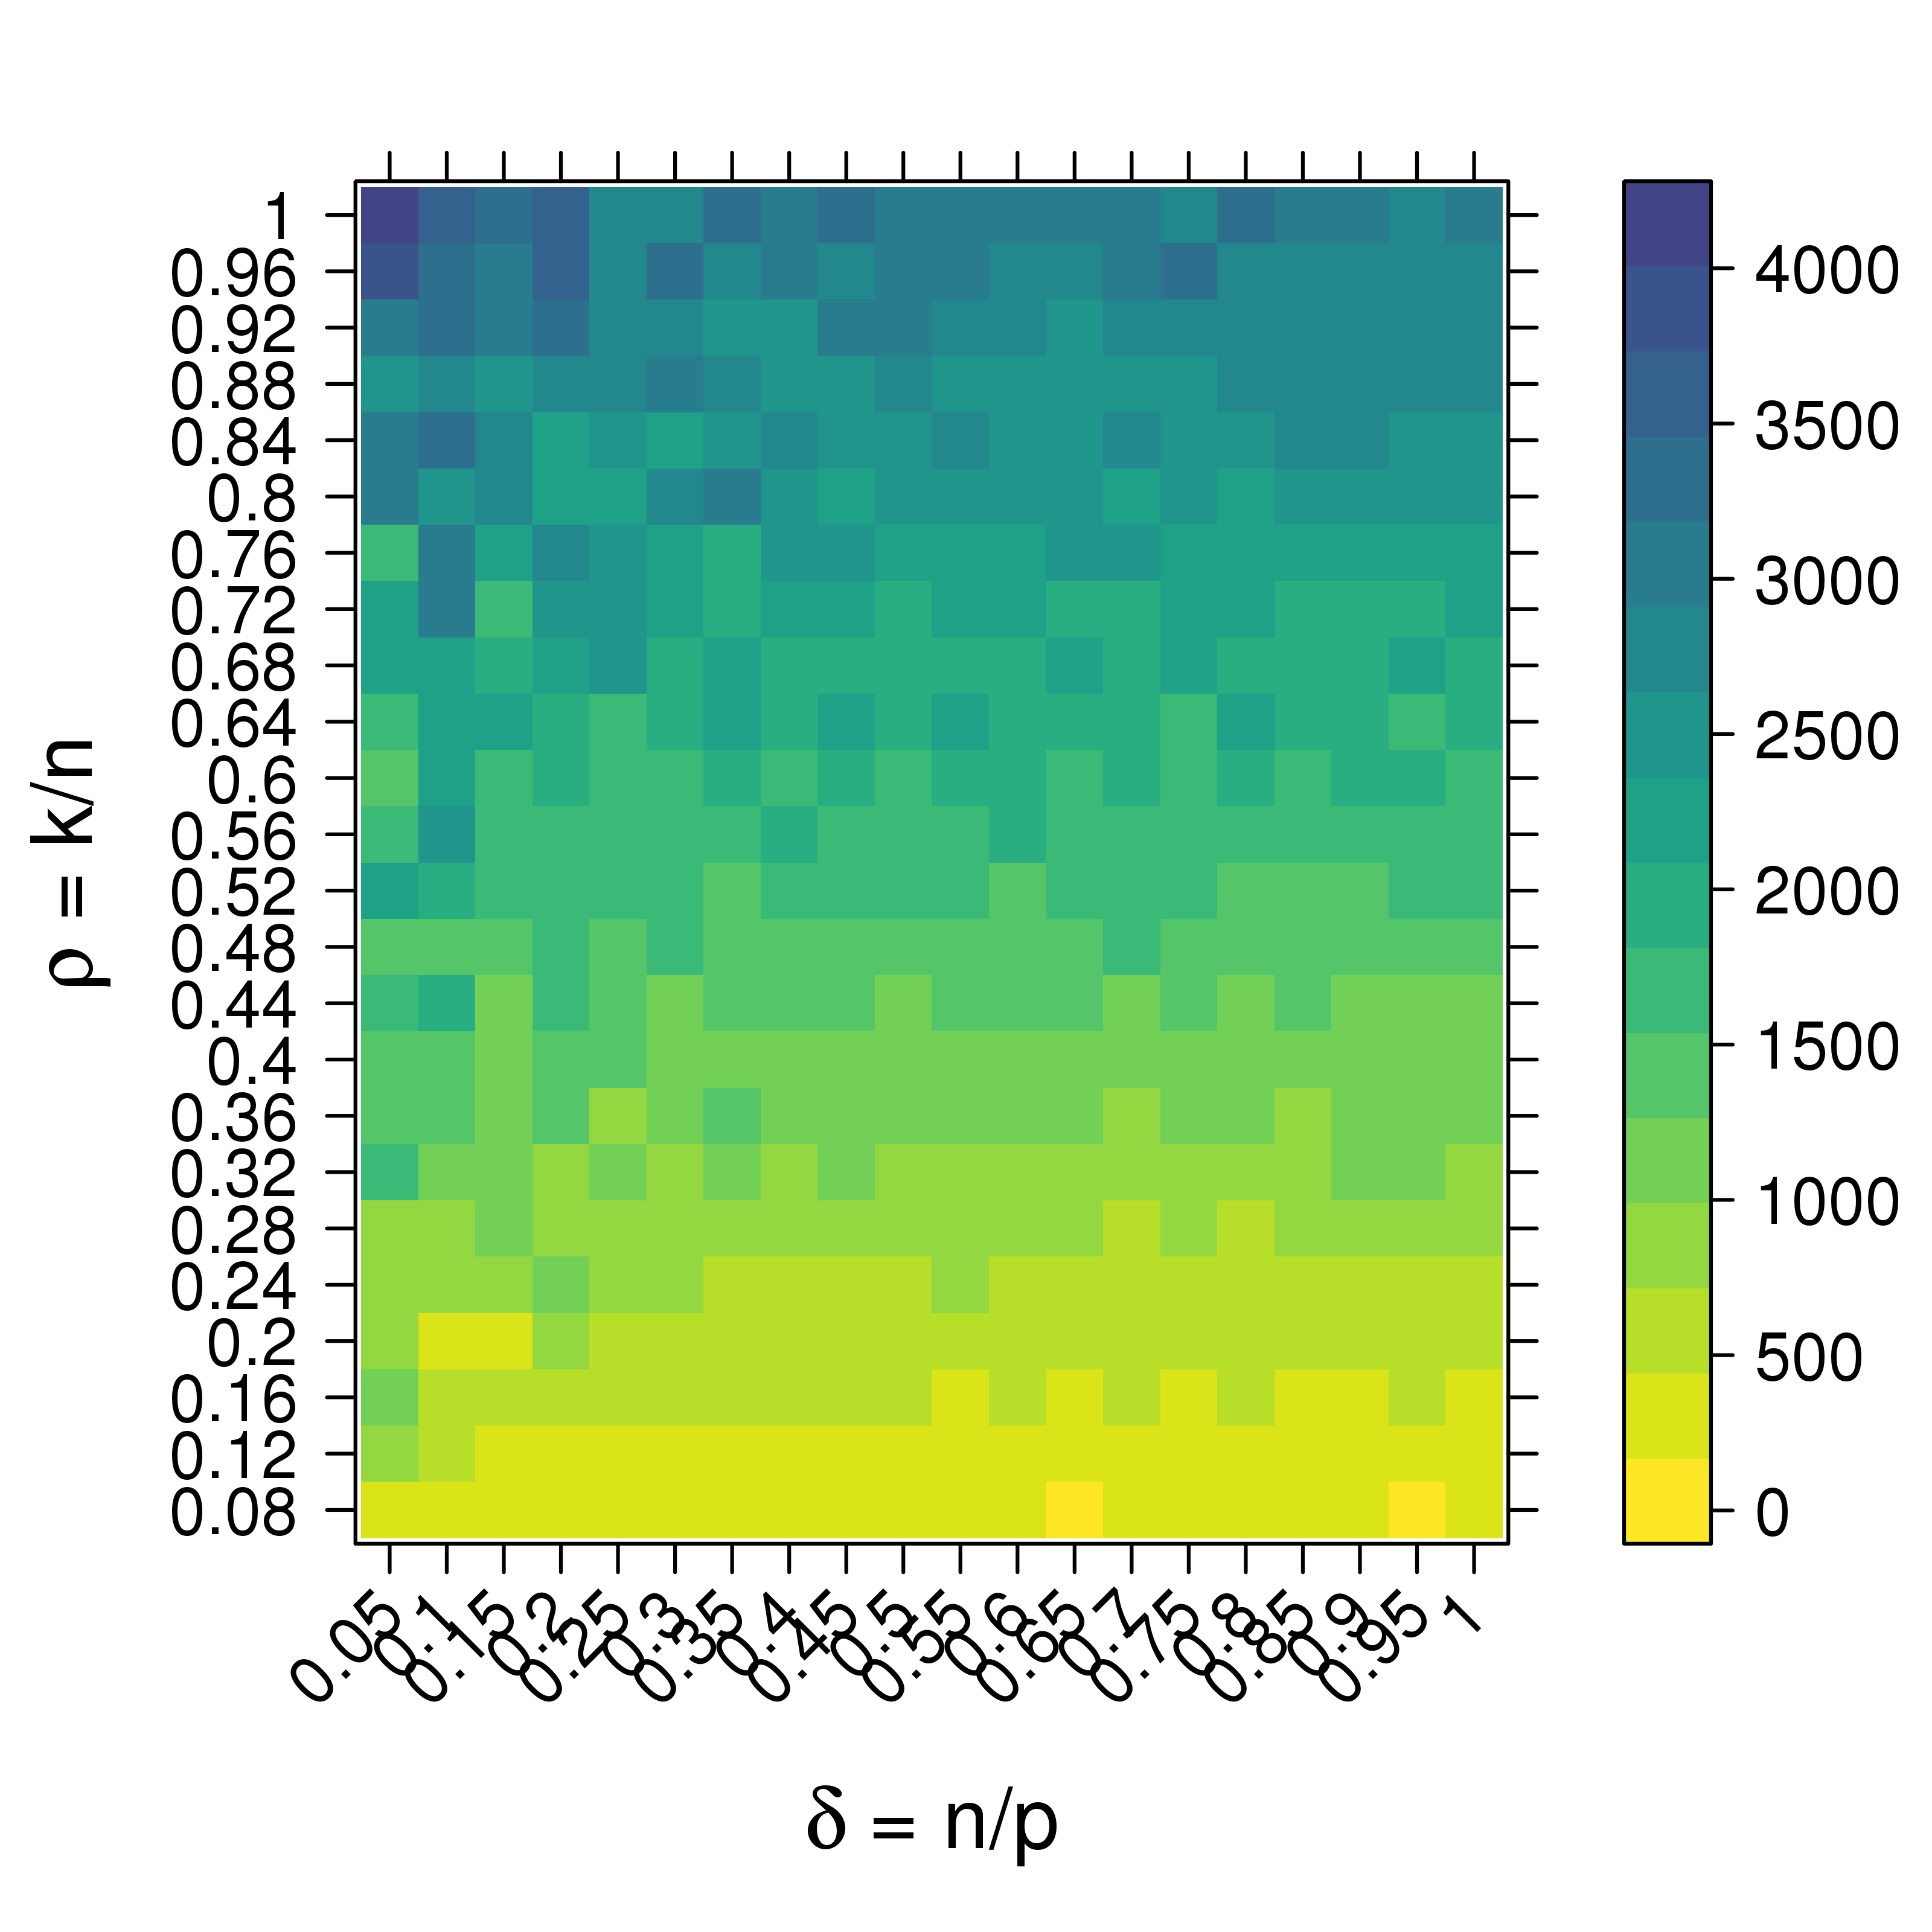
\includegraphics[totalheight=6cm]{./figs/ranger_error_Stodden_simulation.png}
%       \caption{The OOB error rate.}
%       \label{figure:ranger_error_Stodden_simulation.png}
%       \vspace{4ex}
%     \end{subfigure} 
%     \begin{subfigure}[t]{0.5\linewidth}
%       \centering
%       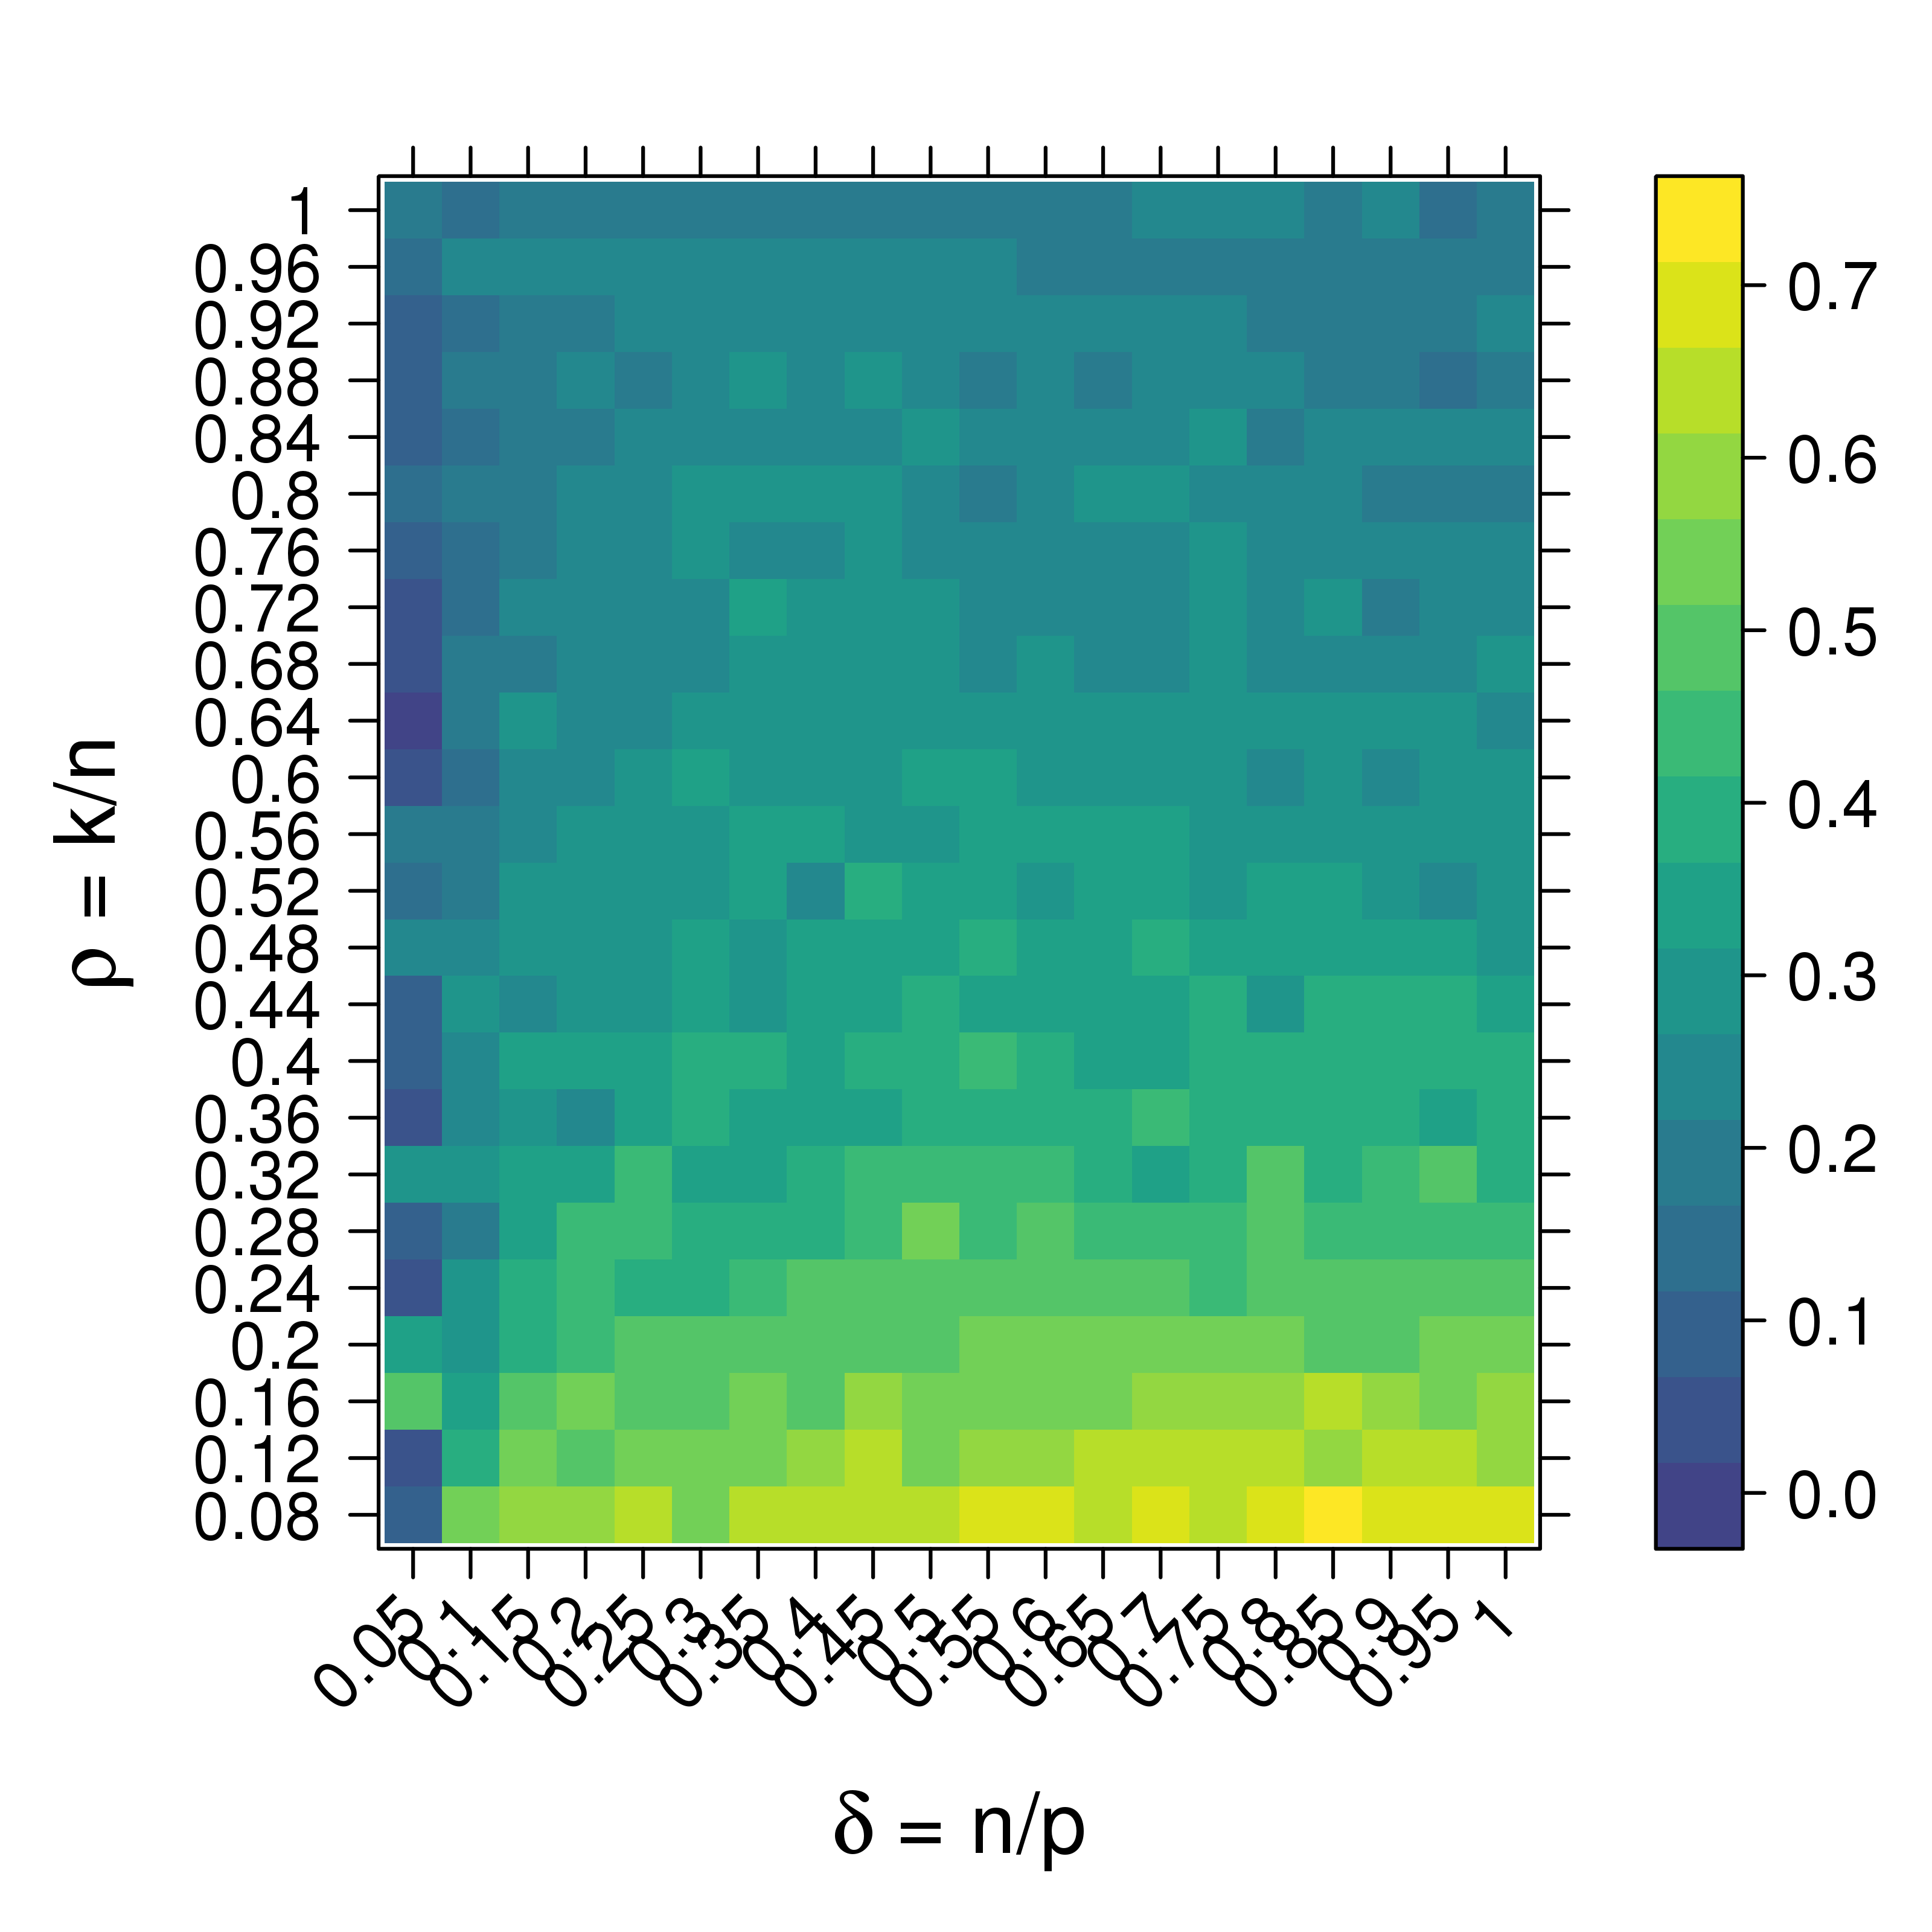
\includegraphics[totalheight=6cm]{./figs/ranger_rbo_Stodden_simulation.png}
%       \caption{The RBO measure}
%       \label{figure:ranger_rbo_Stodden_simulation.png}
%     \end{subfigure} 
%     \caption{The simulated data of \protect{\cite{Donoho.and.Stodden.2006}} with a random forest model.}
%     \label{figure:ranger_error_and_rbo_Stodden_simulation.png}
%%   \end{adjustwidth}
% \end{figure}
%
%
%We have seen no work on the question of such a phase transition in the case of classification problems. Still it may be
%instructive to consider the implications of the phase transition for our work. 
%
%We have used a random forest on the same simulation data used for figure \ref{figure:error_and_rbo_Stodden_FDR.png}.  The
%Donoho-Tanner phase transition arises in recovering the $\beta$ in data generated by a linear model. However, in a
%decision tree (random forest) we are fitting a non-linear model and there is no notion of estimating the
%$\beta$. Because of this we have evaluated the performance of the random forest using the RBO measure on the variable
%importance.
%
%We note that while a random forest is a long way from an all-subsets search, it is a limited search of
%the feature space. As such it may perform outside of the bounds of the phase transition. 
%
%
%Fig~\ref{figure:ranger_error_and_rbo_Stodden_simulation.png} shows the OOB prediction error and the RBO error for a
%random forest with 10000 trees and the \mtry value set to the default for a regression problem (depending on $n$). It
%shows no evidence of following the shape of the Donoho-Tanner phase transition.
%
%As \cursedforest is designed for extremely large numbers of variables it is likely to be operating in difficult regions
%of the figure where the ratio $\delta = n/p$ is small. In the simulated example in section \ref{section:synthetic_data}
%the underdetermination parameter $\delta = 0.002$ and the sparsity parameter $\rho =2\times 10^{-6}.$
%
%The existence of the Donoho-Tanner phase transition is a salutary warning. There are likely to be limits, both
%computational and logical, to the recovery of signals from noisy data. \cursedforest is a contribution to addressing the
%practical limits but the logical limits will still apply. However in the case of data that is both big and wide,
%\cursedforest and other VariantSpark methods may provide a useful tool.


\clearpage
\section{Supporting Information}

% Include only the SI item label in the subsection heading. Use the \nameref{label} command to cite SI items in the text.
%\subsection*{S1 Video}
%\label{S1_Video}
%{\bf Bold the first sentence.}  Maecenas convallis mauris sit amet sem ultrices gravida. Etiam eget sapien nibh. Sed ac ipsum eget %enim egestas ullamcorper nec euismod ligula. Curabitur fringilla pulvinar lectus consectetur pellentesque.


\section*{Acknowledgments}
AO and PS implemented the method, AO conducted the BMD and 1000genomes experiments while PS generated the scaling data,
analysed by RD with input from NE. PL and ELD aided in the interpretatio nof the BMD data, while SL and JD contributed
to the 1000genomes analysis. DCB visualised the BMD and 1000genomes results. All authors contributed to the manuscript.
The authors would like to acknowledge CSIRO, specifically PS, for setting up and maintaining the in-house Spark cluster.

\nolinenumbers

\bibliography{CursedForest}

\end{document}



% We have demonstrated that using a different parallelization model can extend random forests to the case of an
% extremely large number of variables. We have treated the case of variable selection in a $p >> n$ model where most of
% the variables are uninformative and have demonstrated the utility of the model for large GWAS datasets. By comparing
% this implementation to other implementations (including those optimized for large datasets) we have demonstrated the
% utility of this approach.

% Donoho and Tanner \cite{Donoho.and.Tanner.2009} give a ``universal phase change'' result that has applications in a
% large number of areas including variable selection in high dimensions. Consider
% Fig~\ref{figure:phase-diagram-equivalence.png} which shows the region where a model can recover the important variables,
% plotted as a function of $\delta = n/p$ and $\rho =k/n$ (where $k$ is the number of significant variables). There is a
% distinct boundary, shown empirically and also based on arguments from combinatorial geometry, to the region where we can
% reliably recover significant variables.  \cite{Donoho.and.Stodden.2006} investigate the behavior of a number of
% regression approaches for variable selection (LARS, Lasso and forward stepwise) and make the point that above the
% phase-transition line variable recovery is still possible by a combinatorial approach.

% It is not surprising that that it is more difficult to recover the signal variable in the upper-left area of the figure,
% as the problem is both under-determined and sparse. What is surprising is the connection with arguments from
% combinatorial geometry. This suggests that we are seeing a universal rule rather than an implementation issue. As
% \cursedforest is designed for extremely large numbers of variables it is likely to be operating in difficult regions of
% the figure where the ratio $\delta = n/p$ is small.


% We note several things here:
% \begin{itemize}
% \item the Donoho-Tanner phase transition arises in recovering the $\beta$ in data generated by a
%   linear model. However, in a decision tree (random forest) there is no notion of estimating the $\beta$
% \item A decision tree (random forest) is a heuristic search. It may recover a relationship in the space of the
%   combinatorial search.
% \end{itemize}

% The existence of the  Donoho-Tanner phase transition is a salutary warning. There are likely to be limits, both
% computational and logical, to the recovery of signals from noisy data. \cursedforest  is a contribution to addressing the
% practical limits but the logical limits will still apply. However in the case of data that is both big and wide,
% \cursedforest and other VariantSpark methods may provide a useful tool.


% \begin{figure}[tbhp] 
%  \begin{adjustwidth}{-1.00in}{0in}
%     \caption{\textbf{The Donoho-Tanner phase chage diagram.}}
%     \centering
%     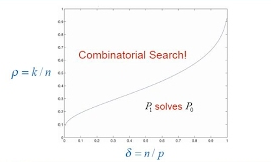
\includegraphics[totalheight=6cm]{./figs/phase.png} 
%     \label{figure:phase-diagram-equivalence.png} 
%     \vspace{4ex}
%   \end{adjustwidth}
% \end{figure}



\begin{figure}[tbhp] 
    \begin{subfigure}[b]{0.5\linewidth}
      \centering
      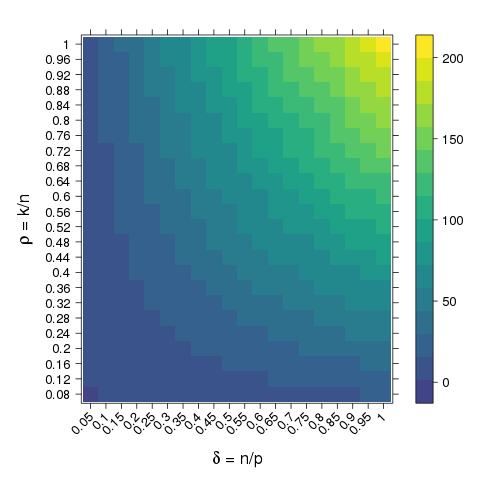
\includegraphics[totalheight=6cm]{./figs/k.png}
      \caption{$k$}
      \label{figure:k.png}
    \end{subfigure} 
    \begin{subfigure}[b]{0.5\linewidth}
      \centering
      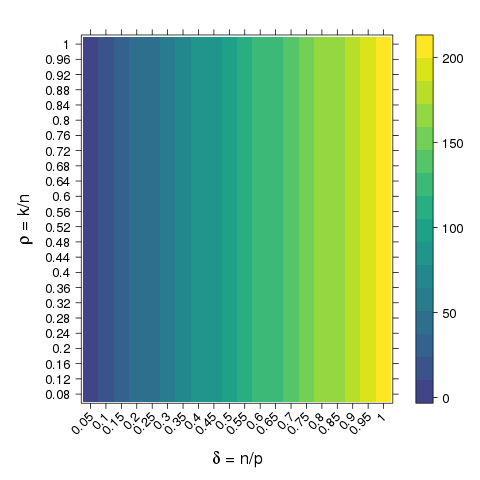
\includegraphics[totalheight=6cm]{./figs/n.png}
      \caption{$n$}
      \label{figure:n.png}
    \end{subfigure} 
    \caption{The simulation in \protect{\cite{Donoho.and.Stodden.2006}} considers $\delta = n/p$ and $\rho =k/n$. Here we plot the
      space of $\{ \delta, \rho$\}, colored  by the parameters $n$ and $k$}
\end{figure}
